%%%%%%%%%%%%%%%%%%%%%%%%%%%%%%%%%%%%%%%%%
% Masters/Doctoral Thesis
% LaTeX Template
% Version 2.3 (25/3/16)
%
% This template has been downloaded from:
% http://www.LaTeXTemplates.com
%
% Version 2.x major modifications by:
% Vel (vel@latextemplates.com)
%
% This template is based on a template by:
% Steve Gunn (http://users.ecs.soton.ac.uk/srg/softwaretools/document/templates/)
% Sunil Patel (http://www.sunilpatel.co.uk/thesis-template/)
%
% Template license:
% CC BY-NC-SA 3.0 (http://creativecommons.org/licenses/by-nc-sa/3.0/)
%
%%%%%%%%%%%%%%%%%%%%%%%%%%%%%%%%%%%%%%%%%

%----------------------------------------------------------------------------------------
%	PACKAGES AND OTHER DOCUMENT CONFIGURATIONS
%----------------------------------------------------------------------------------------

\documentclass[
11pt, % The default document font size, options: 10pt, 11pt, 12pt
%oneside, % Two side (alternating margins) for binding by default, uncomment to switch to one side
%chapterinoneline,% Have the chapter title next to the number in one single line
english, % ngerman for German
singlespacing, % Single line spacing, alternatives: onehalfspacing or doublespacing
%draft, % Uncomment to enable draft mode (no pictures, no links, overfull hboxes indicated)
%nolistspacing, % If the document is onehalfspacing or doublespacing, uncomment this to set spacing in lists to single
%liststotoc, % Uncomment to add the list of figures/tables/etc to the table of contents
%toctotoc, % Uncomment to add the main table of contents to the table of contents
parskip, % Uncomment to add space between paragraphs
%nohyperref, % Uncomment to not load the hyperref package
headsepline, % Uncomment to get a line under the header
]{MastersDoctoralThesis} % The class file specifying the document structure

\usepackage[utf8]{inputenc} % Required for inputting international characters
\usepackage[T1]{fontenc} % Output font encoding for international characters

%\usepackage{palatino} % Use the Palatino font by default

\usepackage[backend=bibtex,natbib=true]{biblatex} % Use the bibtex backend with the authoryear citation style (which resembles APA)

\addbibresource{mpotr.bib} % The filename of the bibliography

\usepackage[autostyle=true]{csquotes} % Required to generate language-dependent quotes in the bibliography

\usepackage{amsmath}
\usepackage{float}
\usepackage[algoruled]{algorithm2e}
\usepackage{tikz}
\usepackage{bytefield}
\usepackage{enumitem}
\usepackage[keys, operators]{cryptocode}
\usepackage{subcaption}


\usepackage{xgreek}
\usepackage{unicode-math}

\setmainfont{CMU Serif}

\usepackage{listings}
\usepackage{color}

\definecolor{mygreen}{rgb}{0,0.6,0}
\definecolor{mygray}{rgb}{0.5,0.5,0.5}
\definecolor{mymauve}{rgb}{0.58,0,0.82}

\lstset{ %
  backgroundcolor=\color{white},   % choose the background color; you must add \usepackage{color} or \usepackage{xcolor}
  basicstyle=\footnotesize,        % the size of the fonts that are used for the code
  breakatwhitespace=true,         	% sets if automatic breaks should only happen at whitespace
  breaklines=true,                 % sets automatic line breaking
  captionpos=b,                    % sets the caption-position to bottom
  commentstyle=\color{mygreen},    % comment style
  frame=single,	                   % adds a frame around the code
  keepspaces=true,                 % keeps spaces in text, useful for keeping indentation of code (possibly needs columns=flexible)
  keywordstyle=\color{blue},       % keyword style
  language=C,                 		% the language of the code
  numbers=left,                    % where to put the line-numbers; possible values are (none, left, right)
  numbersep=5pt,                   % how far the line-numbers are from the code
  numberstyle=\tiny\color{mygray}, % the style that is used for the line-numbers
  rulecolor=\color{black},         % if not set, the frame-color may be changed on line-breaks within not-black text (e.g. comments (green here))
  showspaces=false,                % show spaces everywhere adding particular underscores; it overrides 'showstringspaces'
  showstringspaces=false,          % underline spaces within strings only
  showtabs=false,                  % show tabs within strings adding particular underscores
  stepnumber=1,                    % the step between two line-numbers. If it's 1, each line will be numbered
  stringstyle=\color{mymauve},     % string literal style
  tabsize=4,	                    % sets default tabsize to 4 spaces
  title=\lstname                   % show the filename of files included with \lstinputlisting; also try caption instead of title
}


%Define the myinput macro for algorithm2e
\newlength\mylen
\newcommand\KwExtraIn[1]{%
        \settowidth\mylen{\KwIn{}}%
        \setlength\hangindent{\mylen}%
        \hspace*{\mylen}#1\\}

\newcommand\NextYear{%
  \advance\year by 1 \the\year\advance\year by -1}
\newcommand\PrevYear{%
  \advance\year by -1 \the\year\advance\year by 1}


%----------------------------------------------------------------------------------------
%	MARGIN SETTINGS
%----------------------------------------------------------------------------------------

\geometry{
	paper=a4paper, % Change to letterpaper for US letter
	inner=2.5cm, % Inner margin
	outer=3.8cm, % Outer margin
	bindingoffset=2cm, % Binding offset
	top=1.5cm, % Top margin
	bottom=1.5cm, % Bottom margin
	%showframe,% show how the type block is set on the page
}

%----------------------------------------------------------------------------------------
%	THESIS INFORMATION
%----------------------------------------------------------------------------------------

\thesistitle{Implementation of a Multi-party Off-the-Record messaging protocol} % Your thesis title, this is used in the title and abstract, print it elsewhere with \ttitle
\supervisor{Aristides \textsc{Pagourtzis}} % Your supervisor's name, this is used in the title page, print it elsewhere with \supname
\examiner{} % Your examiner's name, this is not currently used anywhere in the template, print it elsewhere with \examname
\degree{Master of Engineering} % Your degree name, this is used in the title page and abstract, print it elsewhere with \degreename
\author{\mbox{Konsantinos \textsc{Andrikopoulos}}, Dimitrios \textsc{Kolotouros}} % Your name, this is used in the title page and abstract, print it elsewhere with \authorname
\addresses{} % Your address, this is not currently used anywhere in the template, print it elsewhere with \addressname

\subject{Cryptography} % Your subject area, this is not currently used anywhere in the template, print it elsewhere with \subjectname
\keywords{Privacy, Group Messaging, Authentication, Enrytpion, Trancript Consistency, End to End, Surveillance} % Keywords for your thesis, this is not currently used anywhere in the template, print it elsewhere with \keywordnames
\university{\href{http://www.ntua.gr}{National Technical University of Athens}} % Your university's name and URL, this is used in the title page and abstract, print it elsewhere with \univname
\department{\href{http://department.university.com}{School of Electrical and Computer Engineering}} % Your department's name and URL, this is used in the title page and abstract, print it elsewhere with \deptname
\group{\href{http://researchgroup.university.com}{asdf}} % Your research group's name and URL, this is used in the title page, print it elsewhere with \groupname
\faculty{\href{http://faculty.university.com}{Faculty Name}} % Your faculty's name and URL, this is used in the title page and abstract, print it elsewhere with \facname


\hypersetup{pdftitle=\ttitle} % Set the PDF's title to your title
\hypersetup{pdfauthor=\authorname} % Set the PDF's author to your name
\hypersetup{pdfkeywords=\keywordnames} % Set the PDF's keywords to your keywords

\begin{document}

\frontmatter % Use roman page numbering style (i, ii, iii, iv...) for the pre-content pages

\pagestyle{plain} % Default to the plain heading style until the thesis style is called for the body content

%----------------------------------------------------------------------------------------
%	TITLE PAGE
%----------------------------------------------------------------------------------------

\begin{titlepage}
\begin{center}

{\scshape\LARGE \univname\par}\vspace{1.5cm} % University name
\textsc{\Large Diploma Thesis}\\[0.5cm] % Thesis type

\HRule \\[0.4cm] % Horizontal line
{\huge \bfseries \ttitle\par}\vspace{0.4cm} % Thesis title
\HRule \\[1.5cm] % Horizontal line

\begin{minipage}[t]{0.49\textwidth}
\begin{flushleft} \large
\emph{Authors:}\\
\href{http://www.johnsmith.com}{\authorname} \\ % Author name - remove the \href bracket to remove the link
\end{flushleft}
\end{minipage}
\begin{minipage}[t]{0.49\textwidth}
\begin{flushright} \large
\emph{Supervisor:} \\
\href{http://www.jamessmith.com}{\supname} % Supervisor name - remove the \href bracket to remove the link
\end{flushright}
\end{minipage}\\[3cm]

\large \textit{A thesis submitted in fulfillment of the requirements\\ for the degree of \degreename}\\[0.3cm] % University requirement text
\textit{in the}\\[0.4cm]
\deptname\\[2cm] % Research group name and department name

\vfill

{\large \today}\\[4cm] % Date
%\includegraphics{Logo} % University/department logo - uncomment to place it

\vfill
\end{center}
\end{titlepage}

%----------------------------------------------------------------------------------------
%	DECLARATION PAGE
%----------------------------------------------------------------------------------------

%\begin{declaration}
%\addchaptertocentry{\authorshipname}
%
%\noindent We, \authorname, declare that this thesis titled, \enquote{\ttitle} and the work presented in it are our own. We confirm that:
%
%\begin{itemize}
%\item This work was done wholly or mainly while in candidature for a research degree at this University.
%\item Where any part of this thesis has previously been submitted for a degree or any other qualification at this University or any other institution, this has been clearly stated.
%\item Where We have consulted the published work of others, this is always clearly attributed.
%\item Where We have quoted from the work of others, the source is always given. With the exception of such quotations, this thesis is entirely our own work.
%\item We have acknowledged all main sources of help.
%\item Where the thesis is based on work done by us jointly with others, I have made clear exactly what was done by others and what We have contributed ourselves.\\
%\end{itemize}
%
%\noindent Signed:\\
%\rule[0.5em]{25em}{0.5pt} % This prints a line for the signature
%
%\noindent Date:\\
%\rule[0.5em]{25em}{0.5pt} % This prints a line to write the date
%\end{declaration}

\cleardoublepage

%----------------------------------------------------------------------------------------
%	QUOTATION PAGE
%----------------------------------------------------------------------------------------

\vspace*{0.2\textheight}

\noindent\enquote{\itshape Thanks to my solid academic training, today I can write hundreds of words on virtually any topic without possessing a shred of information, which is how I got a good job in journalism.}\bigbreak

\hfill Dave Barry

%----------------------------------------------------------------------------------------
%	ABSTRACT PAGE
%----------------------------------------------------------------------------------------

\begin{abstract}
\addchaptertocentry{\abstractname} % Add the abstract to the table of contents

In a world where the need for easy instant communication must overcome the threat of constant surveillance, end-to-end encryption has become a necessity.
While some protocols enable end-to-end encryption for two parties, there are limited solutions for multiparty end-to-end encryption, particularly for desktop applications.
In this paper we describe the first implementation of mpOTR, the multiparty OTR protocol.
mpOTR achieves confidentiality, authenticity, forward secrecy, deniability, and basic consensus.
The existing theoretical introduction of mpOTR treats the undrelying subprotocols as black boxes and does not describe them in detail.
Our contributions are the complete description of the mpOTR protocol including every subprotocol detail and the first implementation of mpOTR.
Our implementation is a production-grade open source extension of the existing libotr library accompanied by a Pidgin plugin written in C.

  \vspace*{\fill}

{\bf Keywords}: \keywordnames
\end{abstract}

%----------------------------------------------------------------------------------------
%	ACKNOWLEDGEMENTS
%----------------------------------------------------------------------------------------

\begin{acknowledgements}
\addchaptertocentry{\acknowledgementname} % Add the acknowledgements to the table of contents

I would like to thank our supervisor, mr. Aristedes Pagourtzis, for giving me the oportunity to work on this project, and teaching me cryptography.
Nikos Papaspyrou, Dimitris Fotakis, and Vangelis Koukis played a major role in forming my mathematical and programming background.
Without their teachings my academic life would be extremely different.

My partner and co-author, Dimitris, spent a lot of sleepless nights developing the code and solving problems with me or even alone when I couldn't join him.
For this he deserves my gratitude as a person and respect as a software engineer.

Additionaly, this year-long journey wouldn't have met its end without the help of Dionysis Zindros, who guided us and sacrificed a great portion of his time to make sure that our work is finished.

I also can not leave out the Flute protocol's author, George Kadianakis.
My engagement in Flute's development process helped us form a better understanding of the theoretical aspects of secure instant messaging.

I would also like to thank my family, and my friends: Alexis L. and Alexis T., Angeliki, Vasilis K. and Vasilis H., Ilias, Korina, Marilena, Orestis, and Panayiotis.
Without them this thesis would have been completed much sooner.

Finally i must thank the members of the Free Software society of National Technical University of Athens for all the technical and philosophical discussion we had about software development.
\bigbreak
\hfill Andrikopoulos Konstantinos


\end{acknowledgements}

%----------------------------------------------------------------------------------------
%	LIST OF CONTENTS/FIGURES/TABLES PAGES
%----------------------------------------------------------------------------------------

\tableofcontents % Prints the main table of contents

\listoffigures % Prints the list of figures

\listoftables % Prints the list of tables

%----------------------------------------------------------------------------------------
%	ABBREVIATIONS
%----------------------------------------------------------------------------------------

\begin{abbreviations}{ll} % Include a list of abbreviations (a table of two columns)

\textbf{LAH} & \textbf{L}ist \textbf{A}bbreviations \textbf{H}ere\\
\textbf{WSF} & \textbf{W}hat (it) \textbf{S}tands \textbf{F}or\\

\end{abbreviations}

%----------------------------------------------------------------------------------------
%	SYMBOLS
%----------------------------------------------------------------------------------------

\begin{symbols}{ll} % Include a list of Symbols (a three column table)

  $AES_{CTR}$   & AES block cipher in counter mode \\
  $\mathcal{O}$ & Security Adversary \\
  $\mathcal{M}$ & Privacy Adversary \\
  $\mathcal{T}$ & Consensus Adversary \\
  $H$           & A hash function \\
  $\oplus$      & The XOR operation \\
  $\odot$ or $\diamond$ & A generic operation \\

%Symbol & Name & Unit \\

\addlinespace % Gap to separate the Roman symbols from the Greek

\end{symbols}

%----------------------------------------------------------------------------------------
%	DEDICATION
%----------------------------------------------------------------------------------------

\dedicatory{For/Dedicated to/To my\ldots}

%----------------------------------------------------------------------------------------
%	THESIS CONTENT - CHAPTERS
%----------------------------------------------------------------------------------------

\mainmatter % Begin numeric (1,2,3...) page numbering

\pagestyle{thesis} % Return the page headers back to the "thesis" style

% Include the chapters of the thesis as separate files from the Chapters folder
% Uncomment the lines as you write the chapters

%\include{Chapters/Chapter1}
\chapter{Introduction}

\label{chapter:introduction}



%--------------------------------------------

\section{Motivation}
Not much time has passed since Edward Snowden revealed the plans that a certain intelligence agency has for the internet. While the world had always been suspecting that the various 3-letter agencies had the capability of controlling the network at a large scale, everybody was shocked with the confirmation of those suspicions.

In a world where the need for easy instant communication must overcome the threat of constant surveillance, end-to-end encryption has become a necessity. It's not a coincidence that digital privacy has come into focus during the last years. One after another companies advertise the utilization of encryption in their products. Apparently, Instant Messaging is the most favorable means of communication when it comes to end-to-end encryption.

One of the oldest and commonly used protocols that provides privacy in Instant Messaging is the Off-The-Record (OTR). OTR was initially introduced in a paper named "Off-the-Record Communication, or, Why Not To Use PGP" in 2004 \cite{otr} and later improved in \cite{otr_improvedauth}. It was named after the homonymous method of journal sourcing. The primary motivation behind OTR was to provide deniable authentication for the conversation participants while keeping conversations confidential, as in real-life private conversations. The protocol is implemented as a C library and a Pidgin plugin, a user study of which can be found in \cite{otr_userstudy}.

Unfortunately, OTR does only apply in a two-party setting, where only two participants are exchanging messages. However, multi-party chat rooms are also very prominent in everyday communications. A protocol providing the same privacy properties as OTR in a multi-party setting was theoritically described in the "Multi-party Off-the-Record Messaging" paper by I. Goldberg et al. in 2009 \cite{mpotr}. This protocol is called multi-party OTR (mpOTR). Although it's been around since 2009, no actual implementation of mpOTR existed until now.

\section{Our Contributions}
The existing theoretical introduction of mpOTR protocol in \cite{mpotr} treats the underlying subrotocols as black boxes and does not describe them in detail. More specifically, two underlying subprotocols are left unspecified, namely the deniable Authenticated Key Exchange (denAKE) and the Group Key Agreement (GKA). These sub-protocols play a key role in setting up the parameters needed for authentication and encryption.

We propose a full construction for the mpOTR Protocol. We specify every underlying sub-protocol. We also specify all the primitive algorithms used for several cryptographic functions, such as hashing, signing and encrypting. Finally, we propose a detailed low-level description of the protocol, including message structures, encoding, etc.

In addition, we provide the first implementation of mpOTR. Our implementation is a production-grade extension of the existing OTR library accompanied by a pidgin plugin, all writen in C. Both are open source projects, available in our github repositories\footnote{https://github.com/Mandragorian/libotr}\footnote{https://github.com/Mandragorian/pidgin\_otr}. We engineered our implementation in such a way that its security is easily reviewable, and, at the same time, facilitates the free software development model, where contributions in the source code are made from several independent authors.

\section{Outline}
In Chapter \ref{chapter:theoretic_background} we introduce some basic theoretic background. All the concepts, cryptographic primitives, and ideas presented there are essential building blocks of the mpOTR Protocol construction proposed in this thesis.

In Chapter \ref{chapter:threat_model} we specify the threat model of the mpOTR Protocol. We describe the different types of adversaries along with their goals. Then, we describe the goals of the mpOTR Protocol to achieve security against each type of adversary.

In Chapter \ref{chapter:protocol} we present our mpOTR Protocol construction. First, we specify the desirable privacy properties of mpOTR conversations and the underlying network setting. Then, we present a high-level overview of the protocol followed by a detailed description of every building block. Afterwards, we specify several technical details. Finally, we specify the exact structure of the messages exchanged in mpOTR.

In Chapter \ref{chapter:implementation} we present our actual implementation of mpOTR. We introduce  several design challenges and the relevant decisions. Then we present the design model of the mpOTR library. Finally, we specify the Application Programming Interface that our implementation offers to the IM applications in order to utilize mpOTR in group conversations.

In Chapter \ref{chapter:plugin} we present our modifications of the OTR pidgin plugin. We introduce the Graphical User interface and the workflow of a private group conversation.

In Chapter \ref{chapter:related_work} we present other protocols that utilize end-to-end encrpytion in multi-party context.

In Chapter \ref{chapter:future_work} we present several problems regarding specific parts of our mpOTR construction. While our construction is fully functional and secure, solving these problems would enhance the protocol’s privacy and/or usabilty. We fully describe each of them and suggest possible solutions.
\chapter{Theoretic Background}
\label{chapters:TheoreticBackground}

In this chapter we will present some basic theoretic background.
All the concepts, cryptographic primitives, and ideas presented here are essential building blocks of the protocol proposed in this thesis.
As a result before someone carries on forward in this document, she should first have a basic understanding of this chapter.

\subsection{Key Exchange Protocols (KEP)}

The goal of any key exchange protocol is to allow two users to agree on a secret value, known only to them, by exchanging some publicly known information.
This might be counter intuitive at first but as we will see in the next section this goal can be achieved with a very simple construction.

Basically a key exchange protocol is any mechanism that provides two functions.
One of them returns a tuple containing some private and some public information.
The public information returned by that function must be sent to the other so that he can calculate the secret value.
The other accepts the public values of the other user and the private values of this user.
It returns the secret value.

\begin{figure}[H]
  \begin{align*}
    <priv, pub> &= genkey() \\
    secret &= calculate\_secret(priv_i, pub_j)
  \end{align*}
  \caption[The interface of a Key Exchange Protocol]{The KEP interface. $pub_j$ is the public information of user $j$ and $priv_i$ the private information of user $i$.}
\end{figure}

\subsection{\dhname key exchange}

The \dhname key exchange is, as the name suggests, a key exchange protocol.
It plays a major role in our proposed protocol, since it is a building block of many of its components.
In this section we will examine how this KEP is constructed, and what public values must be exchanged.

First, we remind to the readers the operation of multiplication modulo a number, $\oplus$.
We want to multiply two numbers $a$ and $b$ modulo a number $n$, called "the modulo".
This means that we first multiply the two numbers as usual.
Then we calculate the remainder of the result when it is divided by the modulo.
This remainder is the result of the multiplication of those two numbers $a$, $b$ modulo $n$.
This means that if:

\[
  ab = np + r
\]

Then:

\[
  a \oplus b  = r
\]
.

In this section we will also symbolize:

\[
  a^x \equiv a \oplus \dots \oplus a = a^x \mod p
\]

These are all the maths needed to understand how the \dhname key exchange works.
To understand why it is also secure is a whole different matter and we will not cover it in this publication.

The \dhname construction supposes that the two users already agree on two values $g$ and $p$ which are publicly known.
The number $p$ must be prime and is called "the modulo" of the protocol.
The number $g$ is called the "generator" and has the property that for every number $k \in [1 \dots p-1]$ there exists a number $l$ in the same range such that $g^l = k$.

The private information for a user is any random integer $x$ such that $ 1 < x < p$.
The public information is $g^x \mod p$ (any exponentiation from now on will be modulo $p$).

The calculation of the shared secret is trivial.
A user $i$, with private information $x$, and public $g^x$, receives the public information $g^y$ of another user $j$.
He then calculates the value $s = (g^y)^x$ which is the shared secret.
Now note that with $i$'s public information, $j$ can also calculate the same value $s = (g^x)^y$.
The calculated value is the same for the two users since:

\[
  (g^y)^x = (g^x)^y = g^{xy}
\]

In algorithm \ref{algo:dh_genkey} we see the $genkey$ function, and in algorithm \ref{algo:dh_calculate_secret} the $calculate\_secret$ function.

From now on, the public and private information of a user will be called public and private keys accordingly.

\begin{algorithm}[h]
  \KwResult{The private and public information needed by the protocol}
  \Begin{
    x := $random_in_range(1,p-1)$

    p := $g^x$

    \Return{$<x, p>$}
  }
  \caption{The $genkey$ function}
  \label{algo:dh_genkey}
\end{algorithm}

\begin{algorithm}[h]
  \KwIn{$g^y$: the public value of the other user, $x$: the secret value of the user calling the function}
  \KwResult{The shared secret, which is known only to the two users}
  \Begin{
    \Return{$(g^y)^x$}
  }
  \caption{The $genkey$ function}
  \label{algo:dh_calculate_secret}
\end{algorithm}

\section{Man-in-the-Middle attacks}

\dhname is a great protocol for calculating shared secrets it has a grave disadvantage.
Consider the following scenario, where Eve, an evil attacker can control the network so that she can read, drop, and inject packets:

User $i$ wants to privately communicate with user $j$.
She generates a private key $x$ and sends the public key $g^x$ to $j$.

Eve interjects and copies and then drops the packet containing $i$'s public key.
She generates a private key $x\prime$ and the public counterpart $g^{x\prime}$.
She performs a \dhname exchange with $i$'s key and calculates $s_1 = g^{xx\prime}$, since she knows $x\prime$.
She then sends her public key to user $j$.

$j$ believes that the public key he just received belongs to $i$.
He generates his private key $y$, and sends the public key $g^y$ to $i$.
He also calculates $s_2 = g^{yx\prime}$ what he thinks is a shared secret known only to him and $i$.

Eve interjects again to copy and drop the just sent package from the network.
She calculates $s_2 = g^{yx\prime}$, again she knows $x\prime$.
Then she sends her public key $g^{x\prime}$ to $i$, posing as $j$.

Now $i$ receives a public key which she thinks belongs to $j$.
Like $j$ she calculates the shared secret $s_1 = g^{xx\prime}$ which she thinks is only known between her and $j$.

The situation now is that $i$ and $j$ use two different secrets to communicate which are both known to Eve.
Eve can decrypt any message sent by $i$, for example, since she knows $s_i$.
She then can re-encrypt it using $s_2$ and relay it to $j$.

Nor $i$ neither $j$ will be able to know that such tampering is taking place and will continue to communicate, thinking that everything is fine.

The above scenario was described with the \dhname key exchange in mind.
However any similar situation where a malicious attacker can get between two communicating partners who think they are talking directly to each other is known as a Man-in-the-Middle attack.

\section{\tdhname key exchange}

\tdhname is another key exchange protocol.
It is an improvement of \dhname which introduces negligible overhead in the complexity of the protocol.
With doubling length of the first message containing the public keys of a user, this protocol provides both authentication and deniability.

\chapter{Threat Model}
\label{chapters:ThreatModel}

\newcommand{\secadv}{$\mathcal{O}$ }
\newcommand{\privadv}{$\mathcal{M}$ }

In \cite{mpotr} a threat model was specified. First, three adversaries are introduced.

\section{The Adversaries}

\subsection{Security adversary $\mathcal{O}$}
This adversary's goal is to read the messages of the chatroom.
Let $T_c^{\hat{X}}$ be the transcript of chatroom $c$ owned by participant $\hat{X}$.
Then, $\mathcal{O}$ is successful, if he can read any message from transcript $T_c^{\hat{A}}$, where $\hat{A}$ is an honest participant, without receiving it from transcript $T_c^{\hat{X}}$ for any participant $\hat{X}$ where $\hat{X} \ne \hat{A}$.
While $\mathcal{O}$ can, both passively and actively, control the network, decrypt messages sent in other chatrooms and even participate in other sessions, he has limited access on the room he wants to attack.
Not only can he not participate in the session under attack, but he also cannot ask for any secret shared between the participants of the specific room.
He has the ability to inject messages of his liking in the chatroom by asking an, otherwise honest, user.
In essence $\mathcal{O}$ is a somewhat formal definition of the notion of IND-CPA attacks in the multiparty setting.

\subsection{Privacy adversary $\mathcal{M}$}

The privacy adversary aims to break the deniability of the protocol.
He is successful if he can prove to a judge $\mathcal{J}$ that a user $\hat{A}$ participated in, read messages from or authored messages in chatroom $c$.

His restrictions are very few.
He can collaborate with $\mathcal{J}$ before the creation of $c$, participate fully in $c$ and even force $\hat{A}$ to reveal his long term secrets in front of the judge.

\subsection{Consensus adversary $\mathcal{T}$}

\subsubsection{Definition of Consensus}

For two participants $\hat{A}$ and $\hat{B}$, consensus is reached on $T_{C_1}^{\hat{A}}$ when $\hat{A}$ believes $\hat{B}$ claims to have a transcript $T_{C_2}^{\hat{B}}$ such that:

\vbox{%
\begin{itemize}
  \label{consensus_def}
  \item $C_1$ has the same set of participants as $C_2$;
  \item $C_1$ and $C_2$ are the same chat room instance;
  \item $T_{C_2}^{\hat{B}}$ has the same collection of messages as $T_{C_1}^{\hat{A}}$;
  \item $T_{C_2}^{\hat{B}}$ and $T_{C_1}^{\hat{A}}$  agree an each message's origin.
\end{itemize}
}

Notice that the above definition is not symmetric.
This means that $\hat{A}$ can reach consensus with $\hat{B}$ without necessarily $\hat{B}$ reaching consensus with $\hat{A}$.

The interpretation of the term "collection of messages" is intentionally left unclear.
This way, each application can handle the ordering of the messages in different ways.

\subsubsection{$\mathcal{T}$'s goal}

$\mathcal{T}$ is successful when he is able to force an honest user $\hat{A}$ to believe that consensus is reached with another honest user $\hat{B}$ when at least one condition from \ref{consensus_def} does not hold.
Notice that only $\hat{A}$ and $\hat{B}$ must be honest.
$\mathcal{T}$ can otherwise control other users as he sees fit.

\section{The Goals of the Protocol}

The protocol must provide some defence mechanisms against all of the above.

The security adversary \secadv can in no way be successful.
The protocol must ensure that no one outside a chat room can read messages authored for it.
This would be a catastrophic failure.

To defend against the privacy adversary \privadv is also crucial.
One might think, that since an attacker can not read messages, it wont make much difference if they are not deniable.

%\include{Chapters/Chapter4}
\chapter{The Protocol}
\label{chapters:protocol}

%--------------------------------------------

\section{Setup}
\subsection{Offer}
\label{Offer}
During the first phase of the setup procedure, which we call "Offer", the participants calculate a unique session id called $sid_i$. This is a value that will be used to distinguish the current session between other sessions created by the same set of participants. \\

Each participant $\hat{X}$ chooses a random 256-bit value $x_{\hat{X}}$, which is his contribution to the $sid_i$. We define $sid_i$ as the SHA-512 hash of the serialized ordered list that contains every participant's contribution. \\

Each offer message contains the sender's contribution along with his position in the participants list. \\

The participant who wants to initiate the mpOTR protocol, broadcasts an offer message. Once a participant receives an offer message:

\begin{itemize}
	\item[]He checks if the sender's position contained in the message matches his actual position, if not, he rejects the message.

	\item[]He checks if he has already received an offer message from the sender, if so, he rejects the message.

	\item[]He checks if he has already broadcast his own offer message. If not, creates and broadcasts his own offer message.

	\item[]He checks if he has received every participant's contribution. If so, he calculates the $sid_i$ and proceeds to the next setup phase.
\end{itemize}

Notice that these messages are not authenticated and hence the session id must
be verified \emph{after} the participants have exchanged signing keys.


\subsection{Deniable Signature Key Exchange (DSKE)}
\label{DSKE}
In \cite{mpotr} a construction for a DSKE is proposed. Given a deniable
Authenticated Key Exchange\\ (denAKE), two participants of the chat can
generate a deniable and authenticated shared secret. With that secret
they can exchange their ephemeral signing public key in an encrypted and
authenticated fashion, using symmetric algorithms.\\

This is done for every pair of participants. After that, they will all have
created an association table, which associates each participant with their
signing key. Afterwards, the participants must make sure that they all have
constructed the same association table. This is done by each participant
transmitting the hash of the association table (which is sorted in
lexicographical order according to each participant's username). The hash
is signed by the ephemeral signing key. \\

Each participant must verify the signatures in each hash received and also
make sure that each hash is the same with the one he has calculated. If everything
checks out, then he is assured that the association table is the same.

\subsubsection{denAKE}


In \cite{mpotr} no denAKE is specified. We propose the following protocol:

\begin{itemize}

	\item[] Each participant generates a private/public Diffie-Hellman keypair $(A_i, g^{A_i})$, which will be used as a longterm key to idenitfy him to other participants. This
is done only once, when a member first used the protocol, then the key remains
the same for subsequent runs of the protocol.

	\item[] To initiate a denAKE, each participant creates an ephemeral Diffie-Hellman keypair
		$(a_i,g^{a_i})$ used only in this run of the protocol (he uses however the same ephemeral key
		to communicate with all the participants).

	\item[] Then he broadcasts the public components of the longterm and ephemeral keys to
		all chat participants in the tuple $(g^{A_i}, g^{a_i})$. We shall call this
		message a "Handshake Message".

	\item[] When participant $i$ has received a handshake Message $(g^{A_j}, g^{a_j})$ from some
		other participant $j$, she can compute the shared secret, as specified by the triple
		Diffie-Hellman protocol. This secret is $g^{a_ia_j} || g^{A_ia_j} || g^{A_ja_i}$
		.

	\item[] After computing the shared secret she encrypts and mac's a magic number and sends it
		to the other party. This is done to verify that the other party has indeed generated
		the same shared secret and is not an adversary trying to break the forward secrecy
		property of triple Diffie-Hellman, see \ref{confirm_message_explain}. We shall call
		this message a "Confirm Message".

	\item[] When she herself has received the corresponding Confirm Message she is assured that
		the shared secret can be safely used and there is no foul play. Now she
		encrypts-then-macs her signing public key and sends it to the other party. This
		message is called a "Key Message"


	\item[] When a key message is received he first verifies the message using the same mac.
		If the tag checks out he decrypts the key and adds it in the association table.
\end{itemize}

In figure \ref{den_ake_schematic} a schematic description of the protocol is provided.

\paragraph{Order of the concatenation}
When the shared secret is calculated, three values must be concatenated. Since
concatenation is not commutative the two parties must agree on the order that the
concatenation happens.

This is achieved by compare the values $g^{A_i}$ and $g^{A_j}$. If
$g^{A_i} \le g^{A_j}$ then the shared secret is $g^{a_ia_j} || g^{A_ia_j} || g^{A_ja_i}$
If not then the shared secret is $g^{a_ia_j} || g^{A_ja_i} || g^{A_ia_j}$. That is, the
value that is generated using the highest public key takes precedence during the
concatenation.

In the overview of the algorithm above, it was silently assumed that
$g^{A_i} \le g^{A_j}$.

\paragraph{The need of a confirmation message}
\label{confirm_message_explain}
A confirmation message is needed if want to have forward secrecy in this exchange.
We must make sure that we are really speaking with the intended participant. Consider
the following scenario.

An adversary, Eve, creates an ephemeral keypair $(b, g^b)$. Then he poses as Bob to Alice,
and broadcasts a handshake message containing $(g^B,g^b)$ where $g^B$ is Bob's
public longterm key.

After Alice receives the handshake message she can construct the shared secret. Eve
however cannot construct the secret since she does not know Bob's longterm
private key. If Alice starts sending data before confirming that the other party
has indeed arrived at the same secret she is under the danger to lose the forward
secrecy property for all messages she sends with the secret.

Indeed the only reason Eve can't construct the secret that Alice calculated, is
that she doesn't have Bob's longterm private key. This of course means that if
she somehow gets a hold of this key, she can decrypt some messages. This situation
of course does not satisfy the forward secrecy property.


\subsubsection{Properties}

Triple Diffie-Hellman is a protocol that is a) authenticated b) forward secret
and c) deniable.

It is authenticated, because the shared secret can only be calculated by someone
only if he posses one of the longterm private keys (and the corresponding ephemeral
of course).

It is forward secret, because once the ephemeral key has been destroyed, it is
impossible to reconstruct the shared secret even when the longterm
private key is compromised.

It is deniable, because the only values that are exchanged during a protocol run
are the two public keys that a participant will use. Nothing is signed, which means
that nothing can be used to prove that someone took part in a conversation.\\[0.5cm]

Another property of this protocol that comes for free is its very fast key generation
as, basically, any random number can be used as a secret key.

Thus Triple Diffie-Hellman satisfies the properties required in \cite{mpotr} and
can be used as a denAKE.

\begin{figure}[t]
  \fbox{%
    \pseudocode{%
      \textbf{Alice} \< \< \textbf{Bob} \\[][\hline]
      \text{ Choose a random number $x \in Z_p^*$ }\< \< \\
      \< \sendmessageright*{Send \ \left(g^x,g^X\right)} \< \\
      \< \< \text{ Choose a random number $y \in Z_p^*$ } \\
      \< \< s = g^{xy} || g^{Xy} || g^{Yx} \\
      \< \< k_1 = KDF_1(s) \\
      \< \< k_2=KDF_2(s) \\
      \< \sendmessageleft*{Send \ \left(g^y,g^Y\right)} \< \\
      s = g^{xy} || g^{Xy} || g^{Yx} \< \< \\
      k_1 = KDF_1(s) \< \< \\
      k_2 = KDF_2(s) \< \< \\
      \< \sendmessageright*{ Send \\ c = AES_{k_1}("confirm") \\ MAC_{k_2}(c)\ } \< \\
      \< \< \text{Verify mac} \\
      \< \< m = AES^{-1}_{k_1}(c) \\
      \< \< \text{Verify m = "confirm"} \\
      \< \sendmessageleft*{ Send \\ c = AES_{k_1}("confirm") \\ MAC_{k_2}(c)\ } \< \\
      \text{Verify mac} \< \< \\
      m = AES^{-1}_{k_1}(c) \< \< \\
      \text{Verify m = "confirm"} \\
      \< \sendmessageright*{Send \\ c = AES_{k_1}(\pk_a) \\ MAC_{k_2}(c) } \< \\
      \< \< \text{Verify mac} \\
      \< \< \text{Add $\pk_a$ to association table} \\
      \< \sendmessageleft*{Send \\ c = AES_{k_1}(\pk_b) \\ MAC_{k_2}(c) } \< \\
      \text{Verify mac} \< \<  \\
      \text{Add $\pk_b$ to association table} \< \< \\
    }
  }
  \caption{The denAKE protocol, where $X$ and $Y$ are the private parts of the long term keys}
  \label{den_ake_schematic}
\end{figure}

\clearpage
\subsection{GKA}

During this phase the participants derive a shared secret key $g_k$ to be used
as a symmetric encryption key.

The main idea is to compute a combined Diffie-Hellman-like key for all
participants, which will then be used for encryption.

To do this. each participant in the chatroom generates a private exponent.
The shared base is then raised to this exponent. The key agreement begins
by the initiating participant sending his public key to the next participant.

In each step that follows, the participant who just received a list of intermediate
keys from the previous participant must calculate the next intermediate key list and
forward it to the next participant, until the final participant. These messages
shall be called "Upflow Messages".

During the $i$-th iteration, the corresponding participant receives keys from the
$(i - 1)$th participant. and then sends information to the $(i + 1)$th participant.
When the last participant has received the required information, he computes a)the
shared secret and b) the final intermediate key list and then forwards it back to
all previous participants. This message, containing the last intermediate key list
shall be called "Downflow Message".

The other participants now can also caclulate the shared secret and use it for
encryption, using the intermediate key list.

\subsubsection{Detailed description}
For a more detailed description of the protocol we refer to \cite{mpenc}, however
a pseudocode is provided.\\

Algorithm \ref{upflow_algo} presents an overview of how each upflow message is constructed, using the data received from the previous upflow message.\\

Algorithm \ref{downflow_algo} presents an overview of how the final, downflow message is constructed using the data received from the last upflow message.\\


In algorithm \ref{gka_proto_algo} the two previous algorithms (\ref{upflow_algo} and \ref{downflow_algo}) are used in order to execute a complete run of the gka protocol.\\

\begin{algorithm}[H]
	\KwIn{P : participants list}
	\KwExtraIn {InterKeys : previous intermediate key list}
	\KwExtraIn {X : user's secret key}
	\KwExtraIn {N : next participant}
	\KwResult{Sends the new intermediate key list to the next participant}
	\Begin{
	inter\_key\_list := empty\_list

	inter\_key\_list.append( InterKeys.last\_elem() )

	\ForEach{k in InterKeys}
	{
		inter\_key\_list.append( $k^X$ )
	}

	send( N , P || inter\_key\_list)
	}
	\caption{Upflow Message send algorithm}
	\label{upflow_algo}
\end{algorithm}

\vfill
\begin{algorithm}[H]
	\KwIn{P : participants list}
	\KwExtraIn {InterKeys : previous intermediate key list}
	\KwExtraIn {X : user's secret key}
	\KwExtraIn {N : next participant}
	\KwResult{Sends the downflow intermediate key list to the other participants}
	\Begin{
	inter\_key\_list := empty\_list

	\ForEach{k in InterKeys}
	{
		inter\_key\_list.append( $k^X$ )
	}

	inter\_key\_list.reverse()

	send( N , P || inter\_key\_list)
	}
	\caption{Downflow Message send algorithm}
	\label{downflow_algo}
\end{algorithm}

\begin{algorithm}[H]
	\KwIn{P : participants list}
	\KwOut{The shared secret}
	\KwResult{Executes a GKA and produces the shared secret}
	\Begin{

	prev := get\_previous\_participant()

	next := get\_next\_participant()

	x := gka\_genkey()

	\If{prev == NULL}{
		send\_upflow(P, [G], x, next)
		}
	\Else{
			m = receive\_from(prev)

			\If{ m not valid}{
					return error
			}
			\If{ next != NULL}{
				send\_upflow(P, m.key\_list, x, next)
			}
			\Else{
				final\_key := m.key\_list.last\_elem()

				s := $final\_key^x$

				send\_downflow(P, m.key\_list, x)

				return s
			}
	}

	m = wait\_for\_downflow()

	\If{m not valid}{
		return error
	}

	final\_key := m.key\_list[pos]

	s := $final\_key^x$

	return s

	}
	\caption{The GKA protocol}
	\label{gka_proto_algo}
\end{algorithm}

\begin{figure}[H]
  \begin{minipage}{0.49\textwidth}
    \begin{tikzpicture}[scale=.9]
      \def \n {5}
      \def \ndec {4}
      \def \radius {3cm}
      \def \margin {8} % margin in angles, depends on the radius

      \foreach \s in {1,...,\ndec}
      {
        \node[draw, circle] at ({180 + (360/\n * (\s - 1))}:\radius) {$\s$};
        \draw[->, >=latex] ({145 + 36 + (360/\n * (\s - 1))+\margin}:\radius)
          arc ({145 + 36 + (360/\n * (\s - 1))+\margin}:{145 + 36 + 360/\n * (\s)-\margin}:\radius);
      }
      \node[draw, circle] at ({181 + 360/\n * (\n - 1)}:\radius) {$\n$};
    \end{tikzpicture}
    \caption{This diagram demonstrates the upflow of the intermediate keys}
  \end{minipage}
  \begin{minipage}{0.49\textwidth}
    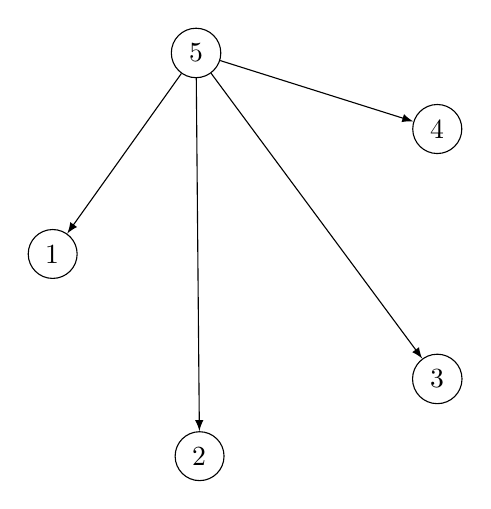
\begin{tikzpicture}[scale=.9]
      \def \n {5}
      \def \ndec {4}
      \def \radius {3cm}
      \def \margin {8} % margin in angles, depends on the radius

      \foreach \s in {1,...,\ndec}
      {
        \node[draw, circle](\s) at ({180 + (360/\n * (\s - 1))}:\radius) {$\s$};
      }
      \node[draw, circle](5) at ({181 + 360/\n * (\n - 1)}:\radius) {$\n$};
      \draw[->, >=latex] (5) -- (1);
      \draw[->, >=latex] (5) -- (2);
      \draw[->, >=latex] (5) -- (3);
      \draw[->, >=latex] (5) -- (4);
    \end{tikzpicture}
    \caption{This diagram demonstrates the downflow of the intermediate keys}
  \end{minipage}
\end{figure}
\subsection{Attest}

During this phase the participants must verify that they agree on the $sid_i$,
and the association table as we mentioned in \ref{Offer} and \ref{DSKE}.
This is needed for two reasons. First because the session id is required before a signing key association table is constructed, and therefore the messages exchanged for the session id calculation can not be signed.
Second because the participants need to verify that they all have the same view of the association table.\\

Each participant calculates the SHA-512 hash of the serialized association table and broadcasts an encrypted and authenticated message that contains both the $sid$ and the calculated hash.
To authenticate the message, the sender uses the ephemeral signing key he has now exchanged with the other participants.
When each participant has received the attest messages from every other participant he must check two things.
He must verify that the hashes of the serialized association table he has received from the other participants are the same with the hash he computed himself.
He also must check that all participants have sent their messages using the same session id.\\

Provided that SHA-512 is a cryptographic hash function an attacker cannot find two signing keys association tables with the same hash.
This means that he is not able to make two participants believe that they have arrived at the same table when they have not.
Also by signing the message with the specific session id, a user implicitly verifies that he is using that particular id for this session.

\section{Communication}

During the communication phase, the participants can exchange authenticated
and encrypted messages using the association table derived from DSKE and the
symmetric encryption key $g_k$ derived from GKA.

\subsection{Origin Authentication}

For origin Authentication we will use public key encryption methods. This is
done because use of symmetric algorithms would require a participant who
wishes to send a message to mac the message $n-1$ times, where $n$ is the
number of the participants.

\subsubsection{Algorithm}

While describing the DSKE we mentioned that an ephemeral signing key is transmitted
by each participant to every other, to be used for message origin verification.

For this purpose we make use of the EdDSA algorithm. This algorithm was selected
for its fast key generation, since a new keypair must be generated in each protocol
run, and its relatively small signature size.

\subsubsection{Signing} \label{signing}

The signature generation is the last step taken before sending a message. This
way we can sign all the properties of the message to be sent, like the $sid$ or the
recipient (if any). We also avoid any manifestations of the Cryptographic Doom
Principle, which states that if a protocol tries to perform \emph{any}
cryptographic operation before verifying the signature or mac on a received
message, it will somehow fail catastrophically and lead to doom.

Symmetrically the signature verification is the first thing that happens before
any other operation is performed on the received message (cryptographic or not).

\subsection{Encryption}

For encryption a shared secret key is used by all the members. This is not a
problem since the origin authentication is provided by the signatures, and
we obviously don't mind any chat member to read a message or we wouldn't
participate in the chat in the first place. For the actual encryption we
use AES-128 in CTR mode.

The use of the CTR mode however has a small pitfall. We must not let the same
nonce be used twice. This is very difficult to achieve in a distributed setting
like a multi-party chat protocol. Despite this we can solve the problem quite
easily. We maintain our original idea of a shared master key, but we don't use
it directly for encryption. Each participant uses the master key and his id in
the chatroom, in order to compute his "personal" encryption key. This encryption
key for participant $p$ is derived as follows:

\[
    K_e = H(ID_p || Key_m)
\]

Provided that $H$ is a cryptographic hash function, an adversary cannot recover
the value $K$ used for encryption as long as he doesn't know the master key.

\subsection{Transcript}

In order to execute the shutdown protocol we need to store the transcript of the chatroom.
In reality a seperate transcript is held for the messages from each participant.
The shutdown protocol will then combine all the different transcripts to determine if consensus has been reached.

The transcript is implemented as a linked list. The list is kept sorted in lexicographic order.
When a message is to be added in a transcript list, the list is searched linearly to find the position the new message should be placed.

When user $A$ sends a message he adds that message to the transcript corresponding to himself.
When he receives a message from user $B$ then he adds that message to the transcript corresponding to user $B$.

\section{Shutdown}

During this phase, the participants end the current session and publish their
ephemeral signing keys, to permit modifying the chat transcript. This adds to
the protocol's deniability property. (Notice though, that the protocol is
deniable without publishing the ephemeral signing keys.)

For a session to be terminated, a "Shutdown Message" is sent.
This message signals to other participants that the shutdown phase should be initiated.
It contains the  hash of all the messages sent by the user sending the "Shutdown Message".
When a user receives a "Shutdown Message", he also sends a "Shutdown Message" containing his own messages hash.
If he has already sent his "Shutdown Message" then he does nothing new.

When one participant has received a "Shutdown Message" from all other participants he can send a "Digest Message".
This message contains a digest of all the messages in the chat-room and is calculated as follows:
\begin{itemize}
  \item[] Sort the participants using their usernames in lexicographic order.
  \item[] For each participant $i$ (in that order) calculate the hash $h_i = H(S_i)$, where $S_i$ is set of all the messages sent by this user (sorted in lexicographic order).
  \item[] Calculate the digest $h = H(h_1 || h_2 \dots || h_N)$, where N is the number of participants.
\end{itemize}

When one participant receives a "Digest Message" from some other participant he checks whether the two of them agree on the chat-room transcript.
He simply compares the digest he computed locally to the one sent by the other participant.
He deduces that consensus is reached only if the two digests are the same.

When one participant has received a "Digest Message" from every other participant he broadcasts an "End Message".
This message signifies that the sender will not user the channel to send any messages anymore.
As a result when a participant receives an "End Message" from all other participants, he is certain that he can release his signing secret key.
Now anyone who intercepts the released key can forge chat-room messages.
However all the participants will no longer accept messages signed with the released secret key, and thus it cannot be used to impersonate its previous owner.

\section{Putting it all together}
Using the subprotocols described above we have this protocol:

\begin{algorithm}[H]
  \KwIn{$\mathcal{P}$ : participants list}
	\KwResult{Executes a run of the mpOTR protocol}
	\Begin{

  $sid$ := Offer($\mathcal{P}$)

  $\mathcal{S}$ := DSKE($sid$, $\mathcal{P}$)

  $\mathcal{K}$ := GKA($sid$, $\mathcal{S}$, $\mathcal{P}$)

  $\mathcal{T}$ := Communication($sid$, $\mathcal{K}$, $\mathcal{S}$, $\mathcal{P}$)

  $c$ := Shutdown($sid$, $\mathcal{T}$, $\mathcal{S}$, $\mathcal{P}$)

  \If{$c$ = "consensus"}{
    \Return{"OK"}
  }
  \Else{
    \Return{"Error"}
  }

	}
	\caption{The mpOTR protocol}
	\label{mpotr_algo}
\end{algorithm}

Where $sid$ is the session id, $\mathcal{S}$ is the signing keys association table, $\mathcal{K}$ is the group shared secret, $\mathcal{T}$ is the transcript of the chatroom and finally $c$ s a boolean value which states if consensus has been reached with all participants.

\subsection{Implementation Notice}

The reader should note that while in \cite{mpotr} a chatroom message consistency
check is specified, it is not yet implemented in our protocol. This is done on
purpose since we are still examining the possible optimization in the proposed
method, which is discussed later in this document.

It must also be made clear that at the moment the protocol does not protect
from message reordering, both from an insider or an outsider to the group.

Thus our protocol is at the time vulnerable both to message reordering and replay
attacks. It is also possible for a participant to send different messages to
different participants.

When the shutdown phase is fully implemented the only possible attack would be
to change the order that the messages appear in.

\section{Message consistency in constant space}

In \cite{mpotr} a straightforward approach is followed. In order to check if
each participant has received the same set of messages all the messages from
each user must be stored, and during the shutdown phase be lexicographically
ordered and hashed. While this achieves our purpose it requires $O(M)$ space
where $M$ is the number of messages.

We believe that the same effect can be achieved in constant space by using
cryptographic accumulators. One can find more about this primitive in \cite{accum_def}.

Since such accumulators are collision free but at the same time quasi-commutative,
they are ideal for our purposes. We can feed the accumulator with the incoming
messages in whichever order they arrive at each participant. The quasi-commutative
property guarantees that if two participants have received the same set of messages
then their accumulators will arrive at the same value in the end.

Thus, we have removed the need to store the messages in order to sort them during
the shutdown phase. We only need to store the value of the accumulator which,
of course, is constant.

\section{Participants ordering}

In many cases, the protocol demands some ordering of the participants. For example, in the Offer step of the Setup phase, the sid contributions should be concatenated in some order before hashing them. Same stands for the public signing keys in the association table, during the Attest step. So we define an ordering rule for the participants, that is used whenever an ordering of elements corresponding to participants is needed. \\

Given that the application provides the mpOTR protocol with a unique name describing each participant, we make the convention that every ordering of the participants list is made lexicographically based on that unique name. We also define the position of the participant, as his position in this order, starting counting from zero (0).

\section{Identity Verification}
The identity of a participant is verified during the DSKE phase.
In order for a participant to be verified the fingerprint of his longterm key must be stored in the known fingerprints file, and be explicitly marked as verified.
In our implementation this file is comma separated and is of the form:

\begin{verbatim}
<account_name>,<protocol>,<buddy_name>,<fingerprint>,<is_verified>
\end{verbatim}

The account name is the "address" of the library user in the form username@host, and is provided by the application.
The protocol is a string that is characteristic of the underlying protocol that the specific account uses.
It is again provided by the application.
The buddy name is the nickname that a user is identified with.
For the time being it is the username part of a users "address".
This implies that the underlying protocol provides addresses which do not change often for a user.
It also means that users from multiple hosts are not allowed or else two users with the same username might conflict.
The above holds for a protocol like jabber for example, but is not the case for protocols like IRC.
As a result our implementation is not fully protocol agnostic at this moment.
Finally the fingerprint is the sha256 hash of the public identity key, and the last field is 1 if the key is verified and 0 otherwise.

This file is read during the plugin start up and initializes the list of all known fingerprints.
When a new chatroom is created, each participant is assigned a list with all known fingerprints used by this participant (from the above list).
When a "Handshake Message" is received the participants known fingerprints list is checked to find (if it exists) a fingerprint matching the currently used public key.
If such a fingerprint is found and it is verified, then the user is verified for this session.
If the found fingerprint is not verified then the participant is not verified.
If no key is found then again the participant is not verified and an entry for this new key is added in the known fingerprints list.

\section{Message Structure}
The general mpOTR message structure is the following: \\

\begin{bytefield}[bitwidth=0.11111\linewidth]{8}
\bitheader{0-7} \\
\begin{rightwordgroup}{Header}
\bitbox{2}{PV} & \bitbox{2}{MT} & \bitbox{4}{Instance Tag} \\
\wordbox{4}{Session ID (64 Bytes)}
\end{rightwordgroup} \\
\wordbox{4}{Payload} \\
\wordbox{2}{Signature}
\end{bytefield} \\

\begin{description}[align=left]
\item [PV] Protocol Version
\item [MT] Message Type
\end{description}

Offer Messages contain no Session ID in the header, since Session ID has not been established yet Offer and DAKE and Shutdown KeyRelease Messages contain no Signature.

\subsection{Offer Message Payload}
\begin{bytefield}[bitwidth=0.11111\linewidth]{8}
\bitheader{0-7} \\
\bitbox{4}{Position} & \bitbox[lrt]{4}{} \\
\wordbox[lr]{1}{Session ID Contribution} \\
\bitbox[l]{4}{} & \bitbox[rb]{4}{} \\
\bitbox[lrb]{4}{}
\end{bytefield}

\subsection{DAKE Handshake Message Payload}
\begin{bytefield}[bitwidth=0.11111\linewidth]{8}
\bitheader{0-7} \\
\bitbox{4}{Ephemeral Key Length} & \bitbox[tlr]{4}{} \\
\wordbox[lr]{1}{Ephemeral Key} \\
\wordbox[blr]{1}{$\cdots$} \\
\bitbox{4}{Longterm Key Length} & \bitbox[tlr]{4}{} \\
\wordbox[lr]{1}{Longterm Key} \\
\wordbox[blr]{1}{$\cdots$}
\end{bytefield}

\subsection{DAKE Confirm Message Payload}
\begin{bytefield}[bitwidth=0.11111\linewidth]{8}
\bitheader{0-7} \\
\bitbox{4}{Recipient} & \bitbox[tlr]{4}{} \\
\wordbox[lr]{1}{Triple Diffie-Hellman MAC} \\
\bitbox[l]{4}{} & \bitbox[rb]{4}{} \\
\bitbox[lrb]{4}{}
\end{bytefield}

\subsection{DAKE Key Message Payload}
\begin{bytefield}[bitwidth=0.11111\linewidth]{8}
\bitheader{0-7} \\
\bitbox{4}{Recipient} & \bitbox[tlr]{4}{} \\
\wordbox[lr]{1}{Triple Diffie-Hellman MAC} \\
\bitbox[l]{4}{} & \bitbox[rb]{4}{} \\
\bitbox[lrb]{4}{} & \bitbox{4}{Key}
\end{bytefield}

\subsection{GKA Upflow Message Payload}
\begin{bytefield}[bitwidth=0.11111\linewidth]{8}
\bitheader{0-7} \\
\bitbox{4}{Recipient} & \bitbox{4}{Key List Length} \\
\bitbox{4}{1st Key Length} & \bitbox[tlr]{4}{} \\
\wordbox[lr]{1}{1st Key} \\
\wordbox[blr]{1}{$\cdots$} \\
\bitbox{4}{2nd Key Length} & \bitbox[tlr]{4}{} \\
\wordbox[lr]{1}{2nd Key} \\
\wordbox[blr]{1}{$\cdots$} \\
\wordbox[blr]{3}{$\cdots$} 
\end{bytefield}

\subsection{GKA Downflow Message Payload}
\begin{bytefield}[bitwidth=0.11111\linewidth]{8}
\bitheader{0-7} \\
\bitbox{4}{Key List Length} & \bitbox{4}{1st Key Length} \\
\wordbox[lr]{1}{1st Key} \\
\wordbox[lr]{1}{$\cdots$} \\
\bitbox{4}{2nd Key Length} & \bitbox[tlr]{4}{} \\
\wordbox[lr]{1}{2nd Key} \\
\wordbox[blr]{1}{$\cdots$} \\
\wordbox[blr]{3}{$\cdots$}
\end{bytefield}

\subsection{Attest Message Payload}
\begin{bytefield}[bitwidth=0.11111\linewidth]{8}
\bitheader{0-7} \\
\wordbox{2}{Session ID (64 Bytes)} \\
\wordbox{2}{Association Table Hash (64 Bytes)} 
\end{bytefield}

\subsection{Data Message Payload}
\begin{bytefield}[bitwidth=0.11111\linewidth]{8}
\bitheader{0-7} \\
\wordbox{1}{CTR} \\
\bitbox{4}{Ciphertext Length} & \bitbox[tlr]{4}{} \\
\wordbox[lr]{1}{Ciphertext} \\
\wordbox[blr]{1}{$\cdots$} \\
\end{bytefield}

\subsection{Shutdown KeyRelease Payload}
\begin{bytefield}[bitwidth=0.11111\linewidth]{8}
\bitheader{0-7} \\
\bitbox{4}{Key Length} & \bitbox[tlr]{4}{} \\
\wordbox[lr]{1}{Key} \\
\wordbox[blr]{1}{$\cdots$} \\
\end{bytefield}
\chapter{Implementation}
\label{chapters:implementation}

%--------------------------------------------

\section{Summary}
Our primary goal was to design and implement the protocol we specified as a production-grade software, aiming to meet the needs of a wide user base. Of course every user would expect such a software to offer privacy in communication between two parties too. That said, implementing mpOTR as part of the OTR library was a natural decision. Not only would this result in a complete IM privacy library, but it would, as well, affect an already existing wide user base.

There exist quite a few implementations of the OTR Library, but only two of them have been actually developed by the OTR Development Team. The first one is implemented in C, it's the very first implementation and the most actively developed having 4 major versions with latest release in March of 2016. The other one is implemented in Java, and has only one release in October of 2009. We chose to develop mpOTR as part of the C implementation of the OTR Library.

\section{Designing the Integration}
Integrating a new feature into an existing software is quite a challenge. Ideally, a good design would at least follow the same coding style, make best reuse of the existing code and follow the same design patters. However, after a carefull inspection of the OTR Library source code we realized that following this approach was unfeasible.

First of all, the coding style in OTR Librady source code is inconsistent. Different characters have been used for indentation, there is no standard error handling style, etc. Reusing parts of the existing code was not an option most of the time due to extensive coupling between the various modules. Finally, no specific design patterns had been used in the existing code.

Our approach was the following. First, we used the coding style used more frequently in the existing code. The code reuse was limitted to the Diffie-Hellman implementation that was the only reusable module of the existing code. As for the design patterns, we decided to use them based on theory.


\section{Design Challenges in C}
A great deal of the callenges a software engineer is going to face when designing a software to be developed in C origins in the lack of literature regarding the Design Patterns. Most of the relative literature, such as the commonly referenced \cite{gofdesignpatterns}, describe the actual implementation of the patterns in the context of an object oriented design.

Given that C is not object oriented, a developer should be innovative when implementing commonly used design patterns. Fortunately, C is a powerfull language offering the mechanisms to implement almost any design pattern. This power mainly comes from two features, the ability to specify incomplete types in order to achieve abstraction in the sense of information hiding, and the use of \textit{void*} in order to achieve generality as interface and inheritence would do in object oriented context. The latter must be carefully used, since it includes type-safety risks.

The most complete reference of design patterns in C can be found in \cite{patternsinc}. Although it only covers a small number of patterns, it gives the reader a clear approach of designing patterns when object-oriented techniques are not natively supported by the language. We also used \cite{patternsinc} as a reference for various patterns we implemented.

\section{Patterns}

\subsection{First-Class ADT}
First-Class ADT is a pattern that decoucples interface from implementation, thus improving encaplulation and providing loose dependencies. We get a definition from \cite{patternsinc}:
\begin{quote}
ADT stands for Abstract Data Type and it is basically a set of values and operations on these values. The ADT is considered first-class if we can have many, unique instances of it.
\end{quote}

We implemented most of the infrastructure modules based on the First-Class ADT pattern, following the implementation paradigm found in \cite{patternsinc}.

The header file of each First-Class ADT contains the declaration of a pointer to an incomplete type and the declaration of all functions that the interface constists of. The source file of each First-Class ADT contains the definition of the incomplete type, as a structure and the definition of each interface function.

Instances of the declared pointer will serve as a handle for the clients. This mechanism enforces the clients to use the provided interface functions rather than directly accessing the fields of the structure.

\subsection{Observer}

\subsection{Iterator}

\section{Idioms}

\section{Naming Conventions}

\chapter{The mpOTR Plugin}
\label{chapters:Plugin}

In addition to the library we also extended the otr pidgin plugin's functionality.
It now uses the extended capabilities of libotr in order to provide private multi-party chatrooms.

Pidgin is an Instant Messaging (IM) client that is compatible with a wide range of IM protocols.
Since our protocol is protocol agnostic\footnote{This is not wholly true. Our implementation of mpOTR assumes that it can send messages of arbitrary length. This is not true in all IM protocols, IRC being one example.} pidgin users can readily chat securely with their existing contacts.

\section{The plugin workflow}

Allow us now to present in summary the workflow of the plugin.

This is what a pidgin chat conversation looks like when no mpOTR session is taking place.
Notice the mpOTR button on the lower right corner, similar to the OTR button.

\includegraphics[scale=0.4]{not_started_unverified.png}

By clicking on the mpOTR button a user has the option to start a private conversation.
If he chooses to do so this is what he sees.

\includegraphics[scale=0.4]{started_unverified.png}

And when some texts are exchanged.

\includegraphics[scale=0.4]{talking_unverified.png}

However, our user (mandragore) hasn't verified another user (mandragore2).
This means that the conversation is unverified.
This is presented to the user in two ways.
First the mpOTR button has a yellow colour and states that the conversation is "Unverified".
And then, the message "You have not verified user: mandragore2".
This message will be displayed for every unverified user.

In order to verify the user mandragore2, our user clicks on the mpOTR button.
Notice how the "Start private conversation" option is now disabled.

\includegraphics[scale=0.4]{click_mpotr_button_unverified.png}

If he clicks the "Verify fingerprints" option this window opens.

\includegraphics[scale=0.4]{verification_ui_opened_unverified.png}

In this window the user can click on the user he wants to verify and (after he checks the fingerprint) click on the "Verify" button.
The selected user will now be verified.

\includegraphics[scale=0.4]{verification_ui_selected_user_unverified.png}

\includegraphics[scale=0.4]{user_verified_unverified.png}

To end the conversation the user clicks on the mpOTR button again and selects the "End private conversation" option.

\includegraphics[scale=0.4]{finished_unverified.png}

Now if the user starts another private conversation the new session will be characterised as "Private".

\includegraphics[scale=0.4]{started_verified.png}


\chapter{Related Work}
\label{chapter:related_work}

As we have already stated, end-to-end encrypted instant messaging is a very trending topic in  the crypto community.
Consequently, a plethora of protocols and implementations achieving the above goal exist, the majority of them handling the two-party case.

Here we will present a brief collection of the aforementioned protocols.
Our goal is not to be exhaustive, but rather to give credit to the authors of those protocols.
Either because their ideas gave us inspiration, or because we experienced first hand the difficulties of implementing and designing secure communication applications, and would like to acknowledge their contributions.

\section{Two-party Protocols}

First we will take a look at protocols providing conversations between two parties.

\subsection{Off-the-Record Messaging}

This protocol could not be missing from this section.
It is designed by the same team which authored the original Multi-part OTR paper \cite{mpotr}.

As far as we know it is the first complete protocol to provide end-to-end encrypted Instant Messaging with strong cryptography.
It set the ground for many other protocols and algorithms, like the axolotl key ratchet, which later evolved into the Signal protocol.

\subsection{Vuvuzela}

\noindent\enquote{\itshape We kill people based on metadata}\bigbreak

\hfill {\small Michael Hayden, former NSA director}
\bigbreak

While end-to-end encryption is an essential component for any privacy protecting protocol, it is not perfect on its own.
The metadata can reveal a bunch of crucial information that can be used to even determine the contents of encrypted data.

Vuvuzela \cite{vuvuzela} is a protocol that provides strong metadata privacy that scales.
It utilizes onion encryption (like TOR) to hide metadata.
Messages are sent in rounds, and noise packets are injected in the network in order to defend against traffic analysis attacks.

\section{Multi-party Protocols}

And now let's see some multi-party protocols.

\subsection{Flute}

Flute is a secure multiparty messaging protocol, currently available as a weechat plugin for irc chatrooms.
It provides end-to-end encryption, but does not offer other desirable properties like deniability or chatroom message consistency.

Flute does not provide everything that is needed for a multi-party protocol to be completely secure.
It's simplicity however, allowed it to have a quick implementation, and also provides the challenge to figure out what protocol are crucial in multi-party messaging, and must be added, or do not really enhance the security and should better be left out.

\subsection{Signal}

Signal, developed by Open Whisper Systems, is currently the most complete solution to the multi-party messaging problem.
It is a robust protocol providing all the necessary properties like \emph{confidentiality, authentication, deniability} and \emph{forward secrecy}.
It does not provide \emph{transcript consistency} but the double-ratchet it uses provides some resistance against reordering attacks.

It is available as an Android and iOS application, and for two party conversation can be used through the chrome browser.
Independently from its authors various applications also use it.
What'sApp, Viber, and Facebook Messenger to name a few, are some of the applications that use the Signal protocol to provide secure chats.
Cryptocat is a firefox plugin that closely follows the Signal approach and is completely open source.

\chapter{Future Work}
\label{chapters:FutureWork}

\section{Message Fragmentation}
Some networks may have a message length limitation that is too small to contain an mpOTR message. To solve this problem, OTR has utilized a fragmentation mechanism since version 2.

The OTR fragmentation mechanism is intuitive. On the sender's side, messages are splitted into a sufficient number of pieces N, so that every fragment does not exceed the specified length limit. Each fragment contains a sequence number k, the value of N and the actual piece. The number k indicates the position of the piece in the whole message, starting from 1 and ending to N. On the recipient's side, the fragments are accumulated so that after receiving the piece with its sequence number k equal to N the whole message can be reconstructed.

This fragmentation mechanism works properly as long as the fragments are delivered in-order. In case of out-of-order delivery the algorithm implements a fragment forgetting strategy that finally rejects the message. A more severe problem arises when fragments from different messages are delivered intermixed. Since each fragment contains no information identifying the message it belongs to, the only distinctive information is the number N. In case N contained in a newly received fragment is different than the one contained in the so far accumulated fragments, the so far accumulated fragments are forgotten. But what happens if fragments from different messages splitted into the same number of pieces N are delivered in an intermixed order? Hopefully, the sequence numbers k won't form a valid sequence. In the extreme scenario the latter happens a non-valid message will be reconstructed.

The problems described above are actually unlikely to happen in a two-party communication context. But such a mechanism in a multi-party context would be a bad choice. Even if fragments are accumulated separately for each sender, there is a sporting chance that fragments from different messages sent during the setup procedure will be delivered intermixed. Rejecting such a message would require a restart of the whole setup procedure, and that could possibly occur indefinitely.

\section{Message consistency in constant space}
In \cite{mpotr} a straightforward approach is followed. In order to check if
each participant has received the same set of messages all the messages from
each user must be stored, and during the shutdown phase be lexicographically
ordered and hashed. While this achieves our purpose it requires $O(M)$ space
where $M$ is the number of messages.

We believe that the same effect can be achieved in constant space by using
cryptographic accumulators. One can find more about this primitive in \cite{accum_def}.

Since such accumulators are collision free but at the same time quasi-commutative,
they are ideal for our purposes. We can feed the accumulator with the incoming
messages in whichever order they arrive at each participant. The quasi-commutative
property guarantees that if two participants have received the same set of messages
then their accumulators will arrive at the same value in the end.

Thus, we have removed the need to store the messages in order to sort them during
the shutdown phase. We only need to store the value of the accumulator which,
of course, is constant.

\section{Message Ordering with OldBlue Protocol}
First let's see what we can and cannot do:
A multi-party chat room is a distributed environment.
This means that there is no central "authority" which can decide if a message came before another.

Also, since we are in a zero trust setting we cannot utilise any values over which the participants have full control, their local clocks for example.

The only information for which we must trust the other participants is what messages they have seen.
We have no other option on this one as we cannot know if an attacker has actually stopped messages from getting to them or if they are dishonest and lie to us.



%----------------------------------------------------------------------------------------
%	THESIS CONTENT - APPENDICES
%----------------------------------------------------------------------------------------

\appendix % Cue to tell LaTeX that the following "chapters" are Appendices

% Include the appendices of the thesis as separate files from the Appendices folder
% Uncomment the lines as you write the Appendices

\setlanguage{monogreek}

\chapter{Περιγραφή Πρωτοκόλλου}
\label{appendices:greek}

Εδώ θα παραθέσουμε μια περιγραφή του πρωτοκόλλου το οποίο υλοποιήσαμε.


\section{Εισαγωγή}
Το Pidgin είναι μια διαδεδομένη εφαρμογή desktop για συνομιλίες πραγματικού χρόνου.
Συνοδεύεται από το OTR πρόσθετο το οποίο, χρησιμοποιώντας το OTR πρωτόκολλο \cite{otr} \cite{otr_improvedauth} \cite{otr_userstudy}, προσθέτει στο Pidgin τη δυνατότητα των από άκρο σε άκρο κρυπτογραφημένων συνομιλιών μεταξύ δύο ατόμων.
Έτσι προσφέρει ασφαλείς συνομιλίες στις οποίες μόνο οι συνδιαλεγόμενοι μπορούν να διαβάσουν τα μηνύματα που ανταλλάσσονται, τα οποία είναι κρυφά ακόμα και στον πάροχο επικοινωνίας.
Παρότι το ίδιο το OTR πρόσθετο προσφέρει συνομιλίες μόνο δύο ατόμων, τα υποβόσκωντα πρωτόκολλα συχνά παρέχουν "δωμάτια" πολλών χρηστών, όπου πολλοί μπορούν να συνομιλούν ταυτόχρονα μεταξύ τους.
Μέχρι τώρα όσοι μιλούσαν σε τέτοιου είδους δωμάτια δεν απολάμβαναν τα πλεονεκτήματα της από άκρο σε άκρο κρυπτογράφησης.

Στόχος της εργασίας μας είναι η υλοποίηση μιας βιβλιοθήκης για ασφαλείς συνομιλίες μεταξύ πολλών ατόμων.
Επιπρόσθετα υλοποιούμε κι ένα πρόσθετο για το Pidgin το οποίο χρησιμοποιεί αυτή τη βιβλιοθήκη έτσι ώστε να επιτρέπει τους χρήστες του Pidgin να συνομιλούν ασφαλώς σε ένα οικείο περιβάλλον.

Η δουλειά μας βασίζεται θεμελιωδώς στο mpOTR paper \cite{mpotr}.
Ακολουθώντας τις συμβάσεις του OTR πρωτοκόλλου, ο όρος "ιδιωτικός" χρησιμοποιείται για να περιγράψει τις ιδιότητες των συνομιλιών της πραγματικής ζωής:

\begin{itemize}
  \item Εμπιστευτικότητα\\
    Μόνο οι συμμετέχοντες μπορούν να διαβάσουν τα μηνύματα\\[0.2cm]

  \item Αυθεντικοποίηση\\
    Οι συμμετέχοντες είναι βέβαιοι ότι πραγματικά μιλάνε σε αυτούς που νομίζουν ότι μιλάνε\\[0.2cm]

  \item Διαψευσιμότητα\\
    Κανείς δε μπορεί να αποδείξει σε κάποιον που δε συμμετείχε στη συνομιλία, ότι κάποιο συγκεκριμένος συμμετέχοντας έλαβε μέρος στη συνομιλία αυτή\\[0.2cm]

  \item Προώθηση Μυστικότητας\\
    Εάν τα μακροπρόθεσμα μυστικά ενός χρήστη εκτεθούν σε κάποιον επιτιθέμενο, τότε αυτός δε μπορεί να διαβάσει κανένα μήνυμα το οποίο στάλθηκε παλαιότερα\\[0.2cm]

\end{itemize}

Όταν έχουμε να κάνουμε για συνομιλίες πολλών ατόμων, μια ακόμα ιδιότητα απαιτείται.
Αυτή η ιδιότητα λέγεται συνέπεια περιεχομένων δωματίου, και γενικά δηλώνει ότι όλοι οι συμμετέχοντες έχουν την ίδια εικόνα για τα μηνύματα που έχουν σταλθεί σε κάποιο δωμάτιο.

Για να υλοποιήσουμε το mpOTR πρωτόκολλο το οποίο περιγράφεται στο \cite{mpotr}, έπρεπε να συγκεκριμενοποιήσουμε τα υπο-πρωτόκολλα τα οποία χρησιμοποιούταν ως μαύρα κουτιά και δεν περιγράφηκαν πλήρως.
Προτείνουμε μια συγκεκριμένη Διαψεύσιμη Ανταλλαγή Κλειδιών Υπογραφής (DSKE) η οποία βασίζεται σε εκτέλεση κατά ζεύγη του τριπλού \dhname πρωτοκόλλου.
Για την Ομαδική Συμφωνία Κλειδιού (GKA) χρησιμοποιούμε το πρωτόκολλο που περιγράφεται στο \cite{mpenc}, αλλά χρησιμοποιούμε κλασσικό \dhname (δηλαδή όχι \dhname ελλειπτικών καμπυλών).

Υλοποιούμε την mpOTR βιβλιοθήκη ως κομμάτι της αρχικής OTR βιβλιοθήκης όπως φαίνεται στο \href{https://github.com/Mandragorian/libotr/tree/mpotr}{το github repo μας\footnote{https://github.com/Mandragorian/libotr/tree/mpotr}}, η οποία μέχρι τώρα πρόσφερε συνομιλίες μόνο για δύο συμμετέχοντες.
Το πρόσθετο μας βασίζεται στο ήδη υπάρχον OTR πρόσθετο το οποίο αναπτύσσεται από την κοινότητα του OTR, και μπορεί κανείς να το δει στο \href{https://github.com/Mandragorian/pidgin_otr/tree/mpotr_integration}{το github repo μας\footnote{https://github.com/Mandragorian/pidgin\_otr/tree/mpotr\_integration}}.
%------------------------------------------------

\section{Το Πρωτόκολλο}

Στον αλγόριθμο \ref{algorithms:mpotr_algo_greek} παρουσιάζουμε τη συμπεριφορά του πρωτοκόλλου.
Το πρωτόκολλο χωρίζεται σε διάφορες φάσεις τις οποίες ονομάζουμε υπο-πρωτόκολλα.
Τα τέσσερα πρώτα από αυτά (Offer, DSKA, GKA και Attest) είναι υπεύθυνα για να κατασκευάσουν όλη την απαραίτητη πληροφορία που απαιτείται ώστε να λάβει χώρα μια ιδιωτική συνομιλία.
Το Communication υπο-πρωτόκολλο είναι αυτό το οποίο αναλαμβάνει να φέρει εις πέρας την ίδια τη συνομιλία.
Τέλος το Shutdown υπο-πρωτόκολλο είναι υπεύθυνο ώστε να γίνει κάθε απαιτούμενη ενέργεια που πρέπει να συμβεί πριν κλείσει μια συνομιλία.
Παρουσιάζουμε εν συντομία τα υπο-πρωτόκολλα αυτά παρακάτω.

Κατά τη διάρκεια του Offer υπο-πρωτοκόλλου, οι συμμετέχοντες υπολογίζουν ένα αναγνωριστικό $sid$ για τη συνομιλία.
Αυτό είναι ένας αριθμός, μοναδικός με μεγάλη πιθανότητα, που ταυτοποιεί τη συνομιλία.

Κατά το DSKE υπο-πρωτόκολλο, κάθε συμμετέχοντας κατασκευάζει έναν πίνακα αντιστοίχησης $\mathcal{S}$ ο οποίος αντιστοιχεί κάθε συμμετέχοντα σε ένα κλειδί υπογραφής το οποίο θα χρησιμοποιηθεί γι αυτή τη συνομιλία.
Κάθε συμμετέχοντας παράγει ένα εφήμερο κλειδί υπογραφής με το οποίο θα αυθεντικοποιεί τα μηνύματά του.
Έπειτα κάθε συμμετέχοντας στέλνει το δημόσιο κομμάτι του κλειδιού υπογραφής του με κάθε άλλο συμμετέχοντα, χρησιμοποιώντας μια Διαψεύσιμη Αυθεντικοποιημένη Ανταλλαγή Κλειδιού (DAKE).
Όταν όλοι έχουν ανταλλάξει τα κλειδιά τους με όλους ο κάθε συμμετέχοντας έχει κατασκευάσει τον πίνακα αντιστοίχισης του.
Αφού η ανταλλαγή κλειδιού είναι διαψεύσιμη, το ίδιο ισχύει και για τα κλειδιά υπογραφής.
Θα μιλήσουμε πιο αναλυτικά για το DSKE και το DAKE στην παράγραφο (\ref{dske_subprot}).

Κατά το GKA υπο-πρωτόκολλο, οι συμμετέχοντες παράγουν ένα κοινό κλειδί $\mathcal{K}$ το οποίο θα χρησιμοποιηθεί για να παραχθούν κλειδιά κρυπτογράφησης.
Τα κλειδιά αυτά θα χρησιμοποιηθούν για να κρυπτογραφηθούν τα μηνύματα που θα σταλούν κατά τη συνομιλία.
Το υπο-πρωτόκολλο αυτό περιγράφεται αναλυτικότερα στην παράγραφο (\ref{gka_subprot}).

Κατά το Attest υπο-πρωτόκολλο οι συμμετέχοντες αυθεντικοποιούν το αναγνωριστικό $sid$ και σιγουρεύονται ότι έχουν φτάσει στον ίδιο πίνακα αντιστοίχισης κλειδιών υπογραφής $\mathcal{S}$.

Κατά το Communication υπο-πρωτόκολλο, λαμβάνει χώρα η ίδια η συνομιλία.
Οι χρήστες χρησιμοποιούν το κοινό μυστικό $\mathcal{K}$, τα εφήμερα κλειδιά υπογραφής και τον πίνακα αντιστοίχισης $\mathcal{S}$, ώστε να κρυπτογραφήσουν και να αυθεντικοποιήσουν τα μηνύματά τους.
Όταν τελειώσει αυτή η φάση παράγεται ένα αντίγραφο της συνομιλίας το οποίο περιέχει όλα τα μηνύματα της συνομιλίας.

Κατά το Shutdown υπο-πρωτόκολλο, οι συμμετέχοντας αποφασίζουν αν υπάρχει συνέπεια περιεχομένων δωματίου και αποκαλύπτουν τα ιδιωτικά κομμάτια των κλειδιών υπογραφής τους.
Εάν τα περιεχόμενα είναι όντως συνεπή τότε λέμε ότι υπάρχει ομοφωνία.
Η αποκάλυψη των ιδιωτικών κλειδιών υπογραφής προσθέτει επιπλέον διαψευσιμότητα στο πρωτόκολλο, όπως και η αποκάλυψη των MAC κλειδιών στο OTR πρωτόκολλο.
Παρόλα αυτά είναι προαιρετικό βήμα καθώς το πρωτόκολλο που προτείνεται είναι διαψεύσιμο και χωρίς την αποκάλυψη.

\begin{algorithm}[t]
  \caption{mpOTR($\mathcal{P}$) --- τρέχει μια συνεδρία του πρωτοκόλλου mpOTR}
  \label{algorithms:mpotr_algo_greek}
    \KwIn{$\mathcal{P}$ : participants list}
  \KwResult{Executes a run of the mpOTR protocol}
  \Begin{

    $sid \leftarrow Offer(\mathcal{P})$

    $\mathcal{S} \leftarrow DSKE(\mathcal{P}, sid)$

    $\mathcal{K} \leftarrow GKA(\mathcal{P}, sid, \mathcal{S})$

    $\mathcal{A} \leftarrow Attest(\mathcal{P}, sid, \mathcal{S})$

    \If{$\mathcal{A}$ = $\perp$}{
      \Return{"Error"}
    }

    $\mathcal{T} := Communication(\mathcal{P}, sid, \mathcal{S}, \mathcal{K})$

    $\mathcal{C} \leftarrow Shutdown(\mathcal{P}, sid, \mathcal{S}, \mathcal{T})$

    \uIf{ConsensusForAll($\mathcal{C}$)}{
      \Return{"OK"}
    }
    \Else{
      \Return{"Error"}
    }
  }

\end{algorithm}

\section{Τα υπο-πρωτόκολλα}
\label{subprots}

Εδώ θα παρουσιάσουμε τα δύο υπο-πρωτόκολλα τα οποία δεν περιγράφονται στο \cite{mpotr}, δηλαδή τη Διαψεύσιμη Ανταλλαγή Κλειδιών Υπογραφής και την Ομαδική Συμφωνία Κλειδιού.

\subsection{DSKE}
\label{dske_subprot}

Στο\cite{mpotr} η ανταλλαγή κλειδιών υπογραφής περιγράφηκε χρησιμοποιώντας ένα πρωτόκολλο που το ονόμαζε ως Διαψεύσιμη Αυθεντικοποιημένη Ανταλλαγή Κλειδιού (DAKE) ως μαύρο κουτί.
Στην υλοποίησή μας χρησιμοποιούμε το τριπλό \dhname πρωτόκολλο ως DAKE, το οποίο είναι αυθεντικοποιημένο και διαψεύσιμο.

Κάθε συμμετέχοντας εκτελεί μια τριπλή \dhname ανταλλαγή κλειδιού με κάθε άλλο συμμετέχοντα στο δωμάτιο και έτσι κατασκευάζουν ένα κοινό μυστικό.
Με αυτό το μυστικό θα κρυπτογραφήσει και έπειτα θα αυθεντικοποιήσει το δημόσιο κομμάτι του κλειδιού υπογραφής του, και θα στείλει το αποτέλεσμα στον άλλον συμμετέχοντα.

Αφού όλοι οι συμμετέχοντας έχουν ανταλλάξει τα κλειδιά υπογραφής τους με όλους τους άλλους, με τον τρόπου που περιγράφηκε παραπάνω, έχουν σχηματίσει τον πίνακα αντιστοίχισης $\mathcal{S}$.
Είναι άξιο να σημειωθεί ότι η DSKE είναι η μόνη φάση κατά την εγκατάσταση της συζήτησης κατά την οποία $O(n^2)$ μηνύματα ανταλλάσσονται.
Μετά στέλνονται $O(n)$ μηνύματα.

Μια σχηματική περιγραφή του πρωτοκόλλου φαίνεται στο σχήμα \ref{den_ake_schematic}.


\subsection{GKA}
\label{gka_subprot}


Για την Ομαδική Συμφωνία Κλειδιού χρησιμοποιούμε το πρωτόκολλο που περιγράφεται στο \cite{mpenc}.
Επαναλαμβάνουμε ότι η βασική ιδέα είναι η \dhname ανταλλαγή κλειδιού, γενικευμένη για πολλούς συμμετέχοντες.

Κατά τη GKA τα μηνύματα ανταλλάσσονται σε δύο φάσεις. Στη φάση της ροής και στη φάση της αντιροής.
Κατά τη φάση της ροής τα μηνύματα ανταλλάσσονται σειριακά μεταξύ των συμμετεχόντων.
Ο κάθε συμμετέχοντας υπολογίζει κάποια ενδιάμεσα κλειδιά, βασιζόμενος στα ενδιάμεσα κλειδιά που έλαβε από τον προηγούμενό του.
Τα ενδιάμεσα κλειδιά αυτά θα τα στείλει στον επόμενο του.
Μετά το πέρας της φάσης ροής, ο τελευταίος συμμετέχοντας έχει αρκετά δεδομένα ώστε να παράξει το κοινό μυστικό.
Επίσης έχει όλη την πληροφορία που χρειάζεται και από τους υπόλοιπους συμμετέχοντες, ώστε να φτιάξουν και αυτοί το κοινό μυστικό.
Αυτή η πληροφορία μεταδίδεται στους υπολοίπους όπως φαίνεται στο σχήμα \ref{figures:gka_downflow}.

Στους αλγορίθμους \ref{upflow_algo_greek}, \ref{downflow_algo_greek}, και \ref{gka_proto_algo_greek} παρουσιάζεται η κεντρική ιδέα της GKA.

\begin{algorithm}[t]
  \caption{SendUpflow($InterKeys$, $x$, $\hat{Y}$) --- στέλνει την νέα λίστα ενδιάμεσων κλειδιών στον επόμενο συμμετέχοντα.}
  \label{upflow_algo_greek}
    \caption{SendUpflow($InterKeys$, $x$, $\hat{Y}$) --- send the new intermediate key list to the next participant.}
  \label{upflow_algo}
  \KwIn {$InterKeys$ : previous intermediate key list}
  \KwExtraIn {$x$ : user's secret key}
  \KwExtraIn {$\hat{Y}$ : the next participant}
  \KwResult{Sends the new intermediate key list to the next participant}
  \Begin
  {
    $inter\_key\_list \leftarrow []$

    $inter\_key\_list.Append(InterKeys.Last() )$

    \ForEach{$k$ in $InterKeys$}
    {
      $inter\_key\_list.Append(k^x)$
    }

    $AuthBroadcast(\hat{Y} \Vert inter\_key\_list)$
  }

\end{algorithm}

\begin{algorithm}[t]
  \caption{SendDownflow($InterKeys$, $x$) --- εκπέμπει την λίστα ενδιάμεσων κλειδιών αντιροής στους υπόλοιπους συμμετέχοντες.}
  \label{downflow_algo_greek}
    \KwIn {$InterKeys$ : previous intermediate key list}
  \KwExtraIn {$x$ : user's secret key}
  \KwResult{Broadcasts the downflow intermediate key list to the other participants}
  \Begin
  {
    $inter\_key\_list \leftarrow []$

    \ForEach{$k$ in $InterKeys$}
    {
      $inter\_key\_list.Append(k^x)$
	}

    $AuthBroadcast(inter\_key\_list)$
  }

\end{algorithm}

\begin{algorithm}[p]
  \caption{GKA($\mathcal{P}$, $sid$, $\mathcal{S}$) - εκτελεί μια Ομαδική Συμφωνία Κλειδιού και παράγει το κοινό μυστικό στο πλαίσιο του συμμετέχοντα $\hat{X}$.}
  \label{gka_proto_algo_greek}
    \caption{GKA($\mathcal{P}$, $sid$, $\mathcal{S}$) - execute a Group Key Agreement and produce the shared secret in the context of participant $\hat{X}$.}
  \label{gka_proto_algo}
  \KwIn{$\mathcal{P}$ : participants list}
  \KwExtraIn{$sid$ : the session ID}
  \KwExtraIn{$\mathcal{S}$ : association table}
  \KwOut{$\mathcal{K}$ : the shared secret}
  \Begin
  {
    $x \leftarrow GenerateKey()$

    $\hat{Y}_{prev} \leftarrow \hat{X}.Previous()$

    $\hat{Y}_{next} \leftarrow \hat{X}.Next()$

    \uIf(\tcc*[f]{$\hat{X}$ is first}){$\hat{Y}_{prev}$ = NULL}
    {
      $SendUpflow([G], x, \hat{Y}_{next})$
    }
    \Else
    {

      \Repeat(\tcc*[f]{wait for previous upflow}){$\hat{R} = \hat{X}$}
      {
        $(\hat{Y}, \hat{R} \Vert key\_list) \leftarrow AuthReceive(\mathcal{S})$
      }

      \If{$\hat{Y}$ $\neq$ $\hat{Y}_{prev}$ $\lor$ $\hat{R} \Vert key\_list = \perp$}
      {
        \Return{error}
      }
      \uIf(\tcc*[f]{$\hat{X}$ is not first or last}){$\hat{Y}_{next}$ $\neq$ NULL}
      {
        $SendUpflow(key\_list, x, \hat{Y}_{next})$
      }
      \Else(\tcc*[f]{$\hat{X}$ is last})
      {
        $final\_key \leftarrow key\_list.Last()$

        $\mathcal{K} \leftarrow final\_key^x$

        $SendDownflow(key\_list, x)$

        \Return{$\mathcal{K}$}
      }
    }

    \Repeat(\tcc*[f]{wait for downflow}){$\hat{Y}$ = $\mathcal{P}.Last()$}
    {
      $(\hat{Y}, key\_list) \leftarrow AuthReceive(\mathcal{S})$
    }
    \If{$key\_list = \perp$}
    {
      \Return{error}
    }

    $pos \leftarrow \mathcal{P}.IndexOf(\hat{X})$

    $final\_key \leftarrow key\_list.Reverse().Get(pos)$

    $\mathcal{K} \leftarrow final\_key^x$

    \Return{$\mathcal{K}$}
  }

\end{algorithm}

\section{Πρωτογενείς Διαδικασίες}

\subsection{Ομάδα Diffie--Hellman}

Στην υλοποίηση μας επαναχρησιμοποιήσαμε τον κώδικα για την ανταλλαγή κλειδιού \dhname από τη βιβλιοθήκη libotr.
Αυτό σημαίνει ότι χρησιμοποιούμε κλασσικό \dhname και συγκεκριμένα την ομάδα υπ. αριθμόν 5 με συντελεστή μήκους 1536 bit.
Στους αλγορίθμους που περιγράψαμε παραπάνω όλες οι υψώσεις σε εκθέτη γίνονται σε αυτή την ομάδα.

\subsection{Κρυπτογράφηση}

Για την κρυπτογράφηση χρησιμοποιούμε AES-128 σε Counter τρόπο λειτουργίας, όπως και στο απλό OTR.
Επιλέξαμε τον AES με κλειδί 128 bit και όχι με 256 αφενός γιατί η ομάδα \dhname που χρησιμοποιούμε δεν παρέχει 256 bit εντροπίας και αφετέρου εξαιτίας διαφόρων μελετών που υποδεικνύουν ότι o αλγόριθμος δρομολόγησης κλειδιού του AES-128 είναι πιο ανθεκτικός σε επιθέσεις \cite{aes-key-recov} \cite{rijndael-improved-analysis}.

Για να κρυπτογραφηθεί ένα μήνυμα, ο χρήστης παραθέτει το κοινό μυστικό με το προσωπικό του αναγνωριστικό για τη συζήτηση και δημιουργεί ένα προσωπικό κλειδί ως εξής:

\[
k_{enc} = H(id_{προσωπικο} || master\ key)
\]

Για τον μετρητή ο κάθε χρήστης διατηρεί τοπικά το δικό του προσωπικό πάνω μισό (τα 8 πιο σημαντικά bytes) το οποίο αυξάνει κατά 1 κάθε φορά που στέλνει ένα μήνυμα.
Το κάτω μισό (8 λιγότερο σημαντικά bytes) είναι πάντα αρχικοποιημένα στο 0.
Σε κάθε μήνυμα που στέλνεται προστίθεται το πάνω μισό του μετρητή.
Το κρυπτοκείμενο παράγεται ως εξής (όπου $ctr$ είναι το πάνω μισό του μετρητή):

\[
ciphertext = AES_{CTR}(k_{enc}, ctr||0, plaintext)
\]

Για να αποκρυπτογραφηθεί ένα μήνυμα, ο χρήστης παραθέτει το κοινό μυστικό με το προσωπικό id του αποστολέα του μηνύματος.

\[
k_{dec} = H(id_{sender} || master\ key)
\]

Και με τον μετρητή που υπάρχει στο μήνυμα αποκρυπτογραφεί ως εξής:

\[
plaintext = AES_{CTR}(k_{dec}, ctr||0, ciphertext)
\]

Αυτό το σχήμα κρυπτογράφησης χρησιμοποιείται ώστε να μην υπάρχει πιθανότητα να επαναχρησιμοποιηθεί κάποια δυάδα μετρητή-κλειδιού κρυπτογράφησης, κάτι που ο Counter τρόπος λειτουργίας απαιτεί να μη συμβεί.

\subsection{Αυθεντικοποίηση}

Για τις υπογραφές χρησιμοποιούμε τον αλγόριθμο EdDSA πάνω στην καμπύλη Ed25519
Κάθε μήνυμα υπογράφεται στο σύνολο του.
Επιλέχτηκε αυτός ο αλγόριθμος για τη γρήγορη παραγωγή κλειδιού αλλά και για το μικρό μήκος υπογραφής.
Αυτό σημαίνει ότι η υπογραφή καλύπτει τόσο τα δεδομένα όσο και τα μέταδεδομένα του μηνύματοσ, όπως το αναγνωριστικό της συνομιλίας, την τιμή του μετρητή και άλλα.

\section{Υλοποίηση}

Θέλοντας να υλοποιήσουμε το mpOTR πρωτόκολλο ως επιπέδου-παραγωγής λογισμικό και στοχεύοντας σε ευρεία βάση χρηστών επιλέξαμε να επεκτείνουμε την ήδη υπάρχουσα OTR βιβλιοθήκη. Σε αυτήν την ενότητα θα παρουσιάσουμε την δομή των επιμέρους συστατικών της υλοποίησης. Θα ακολουθήσουμε μια από πάνω προς τα κάτω προσέγγιση, παρουσιάζοντας πρώτα το συστατικό ανώτατου-επιπέδου και έπειτα τα συστατικά χαμηλότερου επιπέδου.

\subsubsection{Το συστατικό ανώτατου-επιπέδου protocol}
Το συστατικό ανώτατου-επιπέδου της υλοποίησής μας λέγεται \emph{chat\_protocol}. Περιλαμβάνει τα βασικά τελικά σημεία του API που ξεκινούν μία ιδιωτική συνεδρία, διαχειρίζονται τα ληφθέντα ή προς αποστολή μηνύματακαι τερματίζουν μια ιδιωτική συνεδρία. Παρέχει επίσης τελικά σημεία του API για την διαχείριση των ιδιωτικών κλειδιών ταυτοποίησης και την διαχείριση των γνωστών δακτυλικών αποτυπωμάτων των δημόσιων κλειδιών ταυτοποίησης. Εκτενής περιγραφή για το API υπάρχει στην ενότητα \ref{section:api}.

Μεγάλο μέρος της υλοποίησης του πρωτοκόλλου mpOTR πραγματοποιείται κατά την διαχείριση ληφθέντων μηνυμάτων, αφού τότε συμβαίνουν αλλαγές κατάστασης. Όσον αφορά τα ληφθέντα μηνύματα, το συστατικό protocol είναι υπεύθυνο να ελέγχει αν το session ID ταιριάζει, να επιβεβαιώνει τις υπογραφές υπογεγραμμένων μηνυμάτων και τελικά να τα ξεδιαλέγει προωθώντας τα στο κατάλληλο συστατικό υπο-πρωτοκόλλου, προσθέτοντάς τα στην ουρά αναμονής ή απορρίπτοντάς τα. Αφού ένα μήνυμα προωθηθεί σε ένα συστατικό υπο-πρωτοκόλλου, το συστατικό protocol ελέγχει αν έχει συμβεί κάποια αλλαγή κατάστασης και αν χρειάζεται αρχικοποιεί το επόμενο υπο-πρωτόκολλο.

Όσον αφορά τα μηνύματα που πρόκειται να αποσταλούν, είναι υπεύθυνο να ελέγχει αν έχει εγκατασταθεί μια ιδιωτική συνεδρία. Σε αυτήν την περίπτωση πρέπει να τα υπογράψει και να τα κρυπρογραφήσει καταλληλα ή να τα απορρίψει αν συμβεί κάποιο λάθος.

Ο κώδικας του συστατικού protocol παρατίθεται στο παράρτημα \ref{appendices:protocol-code}.

\subsection{Συστατικά υπο-πρωτοκόλλων}
Τα υπο-πρωτόκολλα υλοποιήθηκαν ως ξεχωριστά συστατικά. Η γενική μορφή καθενός περιλαμβάνει μια υλοποίηση ενός First-Class ADT που περιέχει εσωτερικές πληροφορίες του υπο-πρωτοκόλλου. Επίσης παρέχει μια διεπαφή που χρησιμοποιείται από το συστατικό ανώτατου-επιπέδου protocol.

Για κάθε δωμάτιο συνομιλίας, το αντίστοιχο \emph{ChatContextPtr} instance περιέχει ένα handle του First-Class ADT για κάθε υπο-πρωτόκολλο. Τα ληφθέντα μηνύματα προωθούνται απ' το συστατικό ανώτατου-επιπέδου protocol στο κατάλληλο υπο-πρωτόκολλο μαζί με το \emph{ChatContextPtr} instance handle. Το \emph{ChatContextPtr} περιγράφεται στην ενότητα \ref{section:infrastructure-components-greek}.

Κάθε υπο-πρωτόκολλο υλοποιεί τη δική του μηχανή καταστάσεων. Η τρέχουσα κατάσταση παρέχεται από την διεπαφή του First-Class ADT, έτσι ώστε οι αλλαγές κατάστασης να γίνονται αντιληπτές από το συστατικό ανώτατου-επιπέδου protocol.

Ο τύπος του First-Class ADT handle ονομάζεται \emph{Chat[...]InfoPtr} και ο τύπος της κατάστασης \emph{Chat[...]State}, όπου το \emph{[...]} είναι το όνομα του υπο-πρωτοκόλλου.

Η βασική διεπαφή, κοινή στα περισσότερα υπο-πρωτόκολλα, περιλαμβάνει τις κάτωθι συναρτησεις:

\begin{lstlisting}[caption={Γενική διεπαφή υπο-πρωτοκόλλων},label={lst:subprotocol-interface-greek}]
void chat_[...]_info_free(Chat[...]InfoPtr info);
Chat[...]State chat_[...]_info_get_state(Chat[...]InfoPtr info);
int chat_[...]_init(ChatContextPtr ctx, ChatMessage **msgToSend);
int chat_[...]_is_my_message(const ChatMessage *msg);
int chat_[...]_handle_message(ChatContextPtr ctx, ChatMessage *msg, ChatMessage **msgToSend);
\end{lstlisting}

\begin{description}
  \item \emph{chat\_[...]\_info\_free}: Αποδεσμεύει τα εσωτερικά δεδομένα του First-Class ADT που προσδιορίζεται από το \emph{info} handle.

  \item \emph{chat\_[...]\_info\_get\_state}: Επιστρέφει την τρέχουσα κατάσταση του υπο-πρωτοκόλλου που προσδιορίζεται από το \emph{info} handle.

  \item \emph{chat\_[...]\_init}: Αρχικοποιεί ένα υπο-πρωτόκολλο στα πλάισια του δωματίου συνομιλίας που προσδιορίζεται από το \emph{ctx}. Η παράμετρος εξόδου \emph{*msgToSend} επιστρέφει ένα μήνυμα που πρέπει να αποσταλεί μετά την αρχικοποίηση, αν υπάρχει τέτοιο. Επιστρέφει \emph{0} αν δεν συνέβη κάποιο λάθος, \emph{non-zero} σε περίπτβση λάθους. 

  \item \emph{chat\_[...]\_is\_my\_message}: Επιστρέφει \emph{1} αν το μήνυμα πρέπει να διαχειριστεί από αυτό το υπο-πρωτόκολλο ή \emph{0} αν όχι.

  \item \emph{chat\_[...]\_handle\_message}: Διαχειρίζεται το μήνμυα \emph{msg} που ελήφθη στο δωμάτιο συνομιλίας που προσδιορίζεται από το \emph{ctx}. Η παράμετρος εξόδου \emph{*msgToSend} επιστρέφει ένα μήνυμα που πρέπει να αποσταλεί μετά την διαχείριση, αν υπάρχει τέτοιο. Επιστρέφει \emph{0} αν δεν συνέβη κάποιο λάθος, \emph{non-zero} σε περίπτωση λάθους. 
\end{description}

Ο κώδικας των συστατικών υποπρωτοκόλλων παρατίθεται στα παραρτήματα \ref{appendices:offer-code}, \ref{appendices:dske-code}, \ref{appendices:gka-code}, \ref{appendices:attest-code}, \ref{appendices:communication-code} και \ref{appendices:shutdown-code}.

\subsection{Συστατικά υποδομής}
\label{section:infrastructure-components-greek}
Καθένα από τα κάτωθι συστατικά υποδομής περιλαμβάνει την υλοποίησης ενός First-Class ADT συνοδευόμενη από σχετικές συναρτήσεις:

\begin{description}
  \item chat\_context: Περιλαμβάνει ένα First-Class ADT με τύπο handle \emph{ChatContextPtr} που μοντελοποιεί το πλαίσιο ενός δωματίου συνομιλίας. Κάθε instance περιλαμβάνει λεπτομέρειες του δωματίου συνομιλίας (το λογαριασμό χρήστη, το εν χρήσει πρωτόκολλο, τη λίστα συμετεχόντων κτλ.), handles για το info κάθε υπο-πρωτοκόλλου και λεπρομέρειες για την συνεδρία mpOTR (session ID, εφήμερο κλειδί υπογραφής, κοινό μυστικό, κλειδί ταυτοποίησης κτλ.). Επίσης παρέχει συναρτήσεις για την προσθήκη ή την εύρεση ενός context σε μια λίστα contexts.

  \item chat\_message: Παρέχει συναρτήσεις για την δημιουργία κάθε τύπου mpOTR μηνύματος. Κάθε mpOTR μήνυμα μοντελοποιείται ως μια δομή τύπου \emph{ChatMessage}. Επίσης παρέχει συναρτήσεις για σειριοποιίηση και ενός mpOTR μηνύματος και το αντίστροφο.

  \item chat\_participant: Περιλαμβάνει ένα First-Class ADT με τύπο handle \emph{ChatParticipantPtr} που μοντελοποιεί έναν συμμετέχοντα σε ένα δωμάτιο συνομιλίας. Επίσης παρέχει συναρτήσεις για την προσθήκη και την εύρεση ενός συμμετέχοντα σε μια λίστα συμμετεχόντων.
  
  \item chat\_id\_key: Περιλαμβάνει ένα First-Class ADT με τύπο handle \emph{ChatIdKeyPtr} που μοντελοποιεί ένα μακροπρόθεσμο κλειδί ταυτοποίησης του χρήστη. Ο πραγματικός τύπος του κλειδιού ταυτοποίησης μπορεί να είναι οποιοσδήποτε τύπος υλοποιεί την διεπαφή που παρατίθεται στην καταγραφή \ref{lst:internal-key-interface-greek}. Επίσης παρέχει συναρτήσεις για την παραγωγή νέου κλειδιού ταυτοποίησης για έναν λογαριασμό και για την εύρεση ενός κλειδιού ταυτοποίσης σε μια λίστα κλειδιών ταυτοποίησης. Τέλος, παρέχει συναρτήσεις για την ανάγνωση και την εγγραφή μιας λίστας κλειδιών ταυτοποιήσης σε αρχείο.
  
\begin{lstlisting}[caption={Διεπαφή εσωτερικού κλειδιού},label={lst:internal-key-interface-greek}]
struct ChatInternalKeyOps{
    ChatInternalKeyPtr (*generate)(void);
    int (*serialize)(ChatInternalKeyPtr, gcry_sexp_t *);
    ChatInternalKeyPtr (*parse)(gcry_sexp_t);
    unsigned char * (*fingerprint_create)(ChatInternalKeyPtr);
    void (*free)(ChatInternalKeyPtr);
};
\end{lstlisting}

  \item chat\_dh\_key: Ένα First-Class ADT με τύπο handle \emph{ChatDHKeyPtr} που μοντελοποιεί ένα ζεύγος κλειδιών \dhname key και υλοποιεί την διεπαφή εσωτερικού κλειδιού που παρατίθεται στην καταγραφή \ref{lst:internal-key-interface-greek}.

  \item chat\_fingerprint: Περιλαμβάνει ένα First-Class ADT με τύπο handle \emph{OtrlChatFingerprintPtr} που μοντελοποιεί το δακτυλικό αποτύπωμα του δημόσιου κλειδιού ταυτοποίησης ενός συμμετέχοντα. Επίσης παρέχει συναρτήσεις για την εύρεση, την προσθήκη ή την απομάκρυνση ενός δακτυλικού αποτυπώματος από μια λίστα δακτυλικών αποτυπωμάτων. Τέλος, παρέχει συναρτήσεις για την ανάγνωση και εγγραφή μιας λίστας δακτυλικών αποτυπωμάτων σε αρχείο.
  
  \item chat\_pending: Περιλαμβάνει ένα First-Class ADT με τύπο handle \emph{ChatPendingPtr} που μοντελοποιεί ένα εκκρεμές μήνυμα. Κάθε instance περιλαμβάνει το όνομα χρήστη του αποστολέα και την συμβολοσειρά του μηνύματος.
  
  \item chat\_event: Περιλαμβάνει ένα First-Class ADT με τύπο handle \emph{OtrlChatEventPtr} που μοντελοποιεί ένα γεγονός. Κάθε instance περιλαμβάνει τον τύπο του γεγονότος και τα σχετικά με τον τύπο δεδομένα. Παρέχει μια συνάρτηση δημιουργίας γεγονότος για κάθε τύπο γεγονότος.

  \item chat\_info:  Περιλαμβάνει ένα First-Class ADT με τύπο handle \emph{OtrlChatInfoPtr} που μοντελοποιεί τον περιγραφέα ενός δωματίου συνομιλίας και περιλαμβάνει πληροφορίες για ένα συγκεκριμένο δωμάτιο συνομιλίας που αποστέλλονται στην εφαρμογή-πελάτη.
  
  \item{list}: Περιλαμβάνει την υλοποίηση διπλά συνδεδεμένης λίστας και ενός iterator για τη λίστα. Η λίστα υλποιείται ως First-Class ADT με τύπο handle \emph{OtrlListPtr}. Ο iterator επίσης υλοποιείται ως First-Class ADT με τύπο handle \emph{OtrlListIteratorPtr}.
\end{description}


\subsection{Λειτουργικά συστατικά}
Πρόκειται για τα συστατικά που παρέχουν χαμηλού επιπέδου συναρτήσεις. Υπάρχουν τα τρία παρακάτω:

\begin{description}
  \item chat\_sign: Παρέχει συναρτήσεις για παραγωγή και επιβεβαίωση υπογραφών.

  \item chat\_enc: Παρέχει συναρτήσεις για κρυπτογράφηση και αποκρυπτογράφηση.

  \item chat\_serial: Παρέχει συναρτήσεις για σειριοποίηση και αποσειριοποίηση διάφορων τύπων μεταβλητών που χρησιμοποιούνται στα mpOTR μηνύματα.
\end{description}

\section{Επόμενες προσθήκες}

\subsection{Κατάτμηση Μηνυμάτων}
Πολλά δίκτυα θέτουν περιορισμούς για το μήκος του μεταδιδόμενου μηνύματος.
Είναι δυνατόν λοιπόν ένα mpOTR μήνυμα να μη χωρά σε αυτό το μήκος.
Για να λυθεί αυτό το πρόβλημα το OTR χρησιμοποιεί έναν μηχανισμός κατάτμηση από τη δεύτερη έκδοση.

Αυτός ο μηχανισμός είναι αρκετά διαισθητικός.
Από την πλευρά του χρήστη, τα μηνύματα σπάνε σε $Ν$ μικρότερα μηνύματα, το καθένα αρκετά μικρό ώστε να χωρά στο μήκος που επιβάλλεται από το δίκτυο.
Το κάθε κομμάτι περιέχει έναν αριθμό σειράς $k$, τον αριθμό $Ν$ καθώς και ένα κομμάτι του αρχικού, μεγάλου, μηνύματος.
Ο αριθμός $k$ δηλώνει τη θέση του συγκεκριμένου κομματιού στο μεγάλο μήνυμα, ξεκινάει από τον αριθμό 1 και τελειώνει στον $Ν$.
Από την πλευρά του παραλήπτη, τα κομμάτια συγκεντρώνονται έτσι ώστε μόλις ληφθεί το κομμάτι με $k = Ν$, το συνολικό μήνυμα να μπορεί να ανακατασκευαστεί.

Αυτή η μεθοδολογία λειτουργεί, αρκεί τα κομμάτια να παραλαμβάνονται με τη σειρά που στάλθηκαν.
Εάν δεν ισχύει αυτό, το OTR απορρίπτει τα κομμάτια και άρα το συνολικό μήνυμα.
Ένα ακόμα μεγαλύτερο πρόβλημα προκύπτει όταν κομμάτια από διαφορετικά μηνύματα παραλαμβάνονται ανακατεμένα.
Επειδή το κάθε κομμάτι δεν περιέχει κάποια αναγνωριστική πληροφορία για το μήνυμα από το οποίο προέκυψε, το μόνο διακριτικό είναι ο αριθμός $Ν$.
Τι συμβαίνει όμως για δύο διαφορετικά μηνύματα τα οποία σπάνε σε ίδιο αριθμό κομματιών, και τα οποία παραλαμβάνονται ανακατεμένα;

Τα παραπάνω προβλήματα είναι αρκετά απίθανο να συμβούν όταν συνομιλούν δύο άτομα.
Αλλά ένας τέτοιος μηχανισμός για πολλά άτομα θα ήταν κακή επιλογή.
Ακόμα και αν τα κομμάτια συγκεντρώνονται ξεχωριστά για τον κάθε αποστολέα, απόρριψη κομματιού κατά τη φάση εγκατάστασης της συνεδρίας θα απαιτούσε επανεκκίνηση της διαδικασίας, χωρίς εγγυήσεις ότι αυτή τη φορά δε θα πάει κάτι στραβά.

\subsection{Ομοφωνία σε σταθερό χώρο}

Στο \cite{mpotr} ακολουθείται μια "αφελής" λύση.
Για να ελέγχεται η ομοφωνία, τα μηνύματα από κάθε χρήστη αποθηκεύονται μέχρι τη Shutdown φάση, όπου και θα ταξινομηθούν αλφαβητικά και θα περάσουν από μια συνάρτηση κατατεμαχισμού.
Παρότι αυτή η λύση πετυχαίνει το σκοπό του ελέγχου της ομοφωνίας, απαιτεί χώρο μνήμης $O(M)$ όπου $M$ ο αριθμός των μηνυμάτων.

Θεωρούμε ότι μπορούμε να πετύχουμε το ίδιο αποτέλεσμα σε σταθερό χώρο χρησιμοποιώντας κρυπτογραφικούς συγκεντρωτές \cite{accum_def}.

Αφού αυτοί οι συγκεντρωτές είναι ανθεκτικοί στις συγκρούσεις, αλλά παράλληλα και ημι-μεταθετικοί είναι ιδανικοί για τους σκοπούς μας. Μπορούμε να περνάμε στον συγκεντρωτή τα λαμβανόμενα μηνύματα με όποια σειρά αυτά έρχονται. Η ημι-μεταθετικότητά τους μας διασφαλίζει ότι αν δύο συμμετέχοντας λάβουν τα ίδια μηνύματα τότε οι συγκεντρωτές τους θα καταλήξουν στην ίδια τιμή στο τέλος.

Έτσι δεν έχουμε πια την ανάγκη να αποθηκεύουμε τα μηνύματα έτσι ώστε να τα ταξινομήσουμε στη Shutdown φάση. Μας αρκεί μόνο να αποθηκεύουμε την τιμή του συγκεντρωτή, η οποία είναι προφανώς σταθερού χώρου.

\section{Αιτιώδης διάταξη μηνυμάτων}

Εδώ θα δούμε επιφανειακά πώς μπορούμε να πετύχουμε αιτιώδη διάταξη των μηνυμάτων μέσα σε ένα δωμάτιο επικοινωνίας.

\subsection{Γιατί αιτιώδης διάταξη}

Για να καταλάβουμε γιατί η αιτιώδης διάταξη είναι το καλύτερο δυνατό που μπορούμε να πετύχουμε ας δούμε τι μπορούμε και τι δε μπορούμε να κάνουμε:
Πρώτα παρατηρήστε ότι ένα δωμάτιο επικοινωνίας πολλών ατόμων είναι ένα κατανεμημένο περιβάλλον.
Αυτό σημαίνει ότι δεν υπάρχει κάποια κεντρική αρχή, η οποία να μπορεί να αποφασίσει αν ένα μήνυμα ήρθε πριν από κάποιο άλλο.

Ακόμη επειδή κανένας συμμετέχοντας δεν εμπιστεύεται κάποιον άλλον, δε μπορούμε να χρησιμοποιήσουμε τιμές, τις οποίες οι συμμετέχοντες ελέγχουν πλήρως, τα ρολόγια του υπολογιστή τους για παράδειγμα.

Η μόνη πληροφορία που \emph{πρέπει} να εμπιστευτούμε τους άλλους συμμετέχοντες είναι ποια μηνύματα έχουν δει.
Δεν έχουμε άλλη επιλογή εδώ καθώς δε μπορούμε να ξέρουμε αν ένας επιτιθέμενος έχει κόψει μηνύματα, αν ο συμμετέχοντας μας λέει ψέμματα ή αν απλά το μήνυμα έχει καθυστερήσει λόγο δρομολόγησης.

\setlanguage{american}

%\include{Appendices/AppendixB}
%\include{Appendices/AppendixC}

%----------------------------------------------------------------------------------------
%	BIBLIOGRAPHY
%----------------------------------------------------------------------------------------
\printbibliography

%----------------------------------------------------------------------------------------

\end{document}
